\documentclass[sansserif, 10pt]{beamer}
\usepackage{graphicx}
\usepackage{subcaption}
\usepackage{amsfonts}
\usepackage{amsmath}
\usepackage{algorithm2e}
\usepackage{rotating}
\usepackage{/home/sci/weiliu/haldefs}
\usepackage{media9}
\usepackage{tikz}
\usepackage{calligra}

\usetheme{Warsaw}
\useinnertheme{rectangles}

\setbeamertemplate{headline}{} % remove section from header.
\setbeamertemplate{navigation symbols}{}
\renewcommand\mathfamilydefault{\rmdefault}
\renewcommand{\inserttotalframenumber}{52}
\setbeamertemplate{footline}[page number] % add page number
\setbeamerfont{institute}{size=\large}
\setbeamerfont{author}{size=\large}



%% \AtBeginSection[]
%% {
%%   \begin{frame}<beamer>
%%     \frametitle{Outline for section \thesection}
%%     \tableofcontents[currentsection, sectionstyle=show/hide, subsectionstyle=show/show/hide]
%%   \end{frame}
%% }

%% \AtBeginSection[]
%% {
%% \begin{frame}<beamer>{Table of Contents}
%% \tableofcontents[currentsection,currentsubsection, 
%%     hideothersubsections, 
%%     sectionstyle=show/shaded,
%% ]
%% \end{frame}
%% }


\title[Resting-State Functional MRI Analysis by Graphical Model]{Resting-State
  Functional MRI Analysis by~Graphical Model}

\subtitle{With Applications on Functional Network Estimation}
\author[W. Liu]{Wei Liu}
\institute[SCI]{
  Scientific Computing and Imaging Institute\\
  University of Utah\\
  Advisor: Tom Fletcher\\
}
\date{December 18, 2013}
\titlegraphic{
\includegraphics[height=1cm]{sfig/SCI_logo_mono} \hspace{2cm}
\includegraphics[height=1cm]{sfig/ulogo}}
\begin{document}

% 1) fMRI measures the blood oxygenation, and indirectly detect the neuronal
% activity. 2) fMRI have been widely used for the neural basis of the
% perception, cognition and emotion. 3) traditionally has been focusing on the
% regions that shows task-related increases in neural activity. 4) rs-fMRI
% detects the neuronal activity during rest.

% Why interested in resting-state? 1) some regions has greater activity in
% baseline state than during experimental task (DMN) 2) enhance understanding of
% neural activity in baseline states. 3) refine interpretation of activation and
% deactivation.

% mental process. 

% The DMN is only slightly disrupted during passive sensory processing task, but
% is suspended during cognitively demanding external tasks. 

{% use the curly bracket for the range of the backgroundtemplate. 
\usebackgroundtemplate{%
  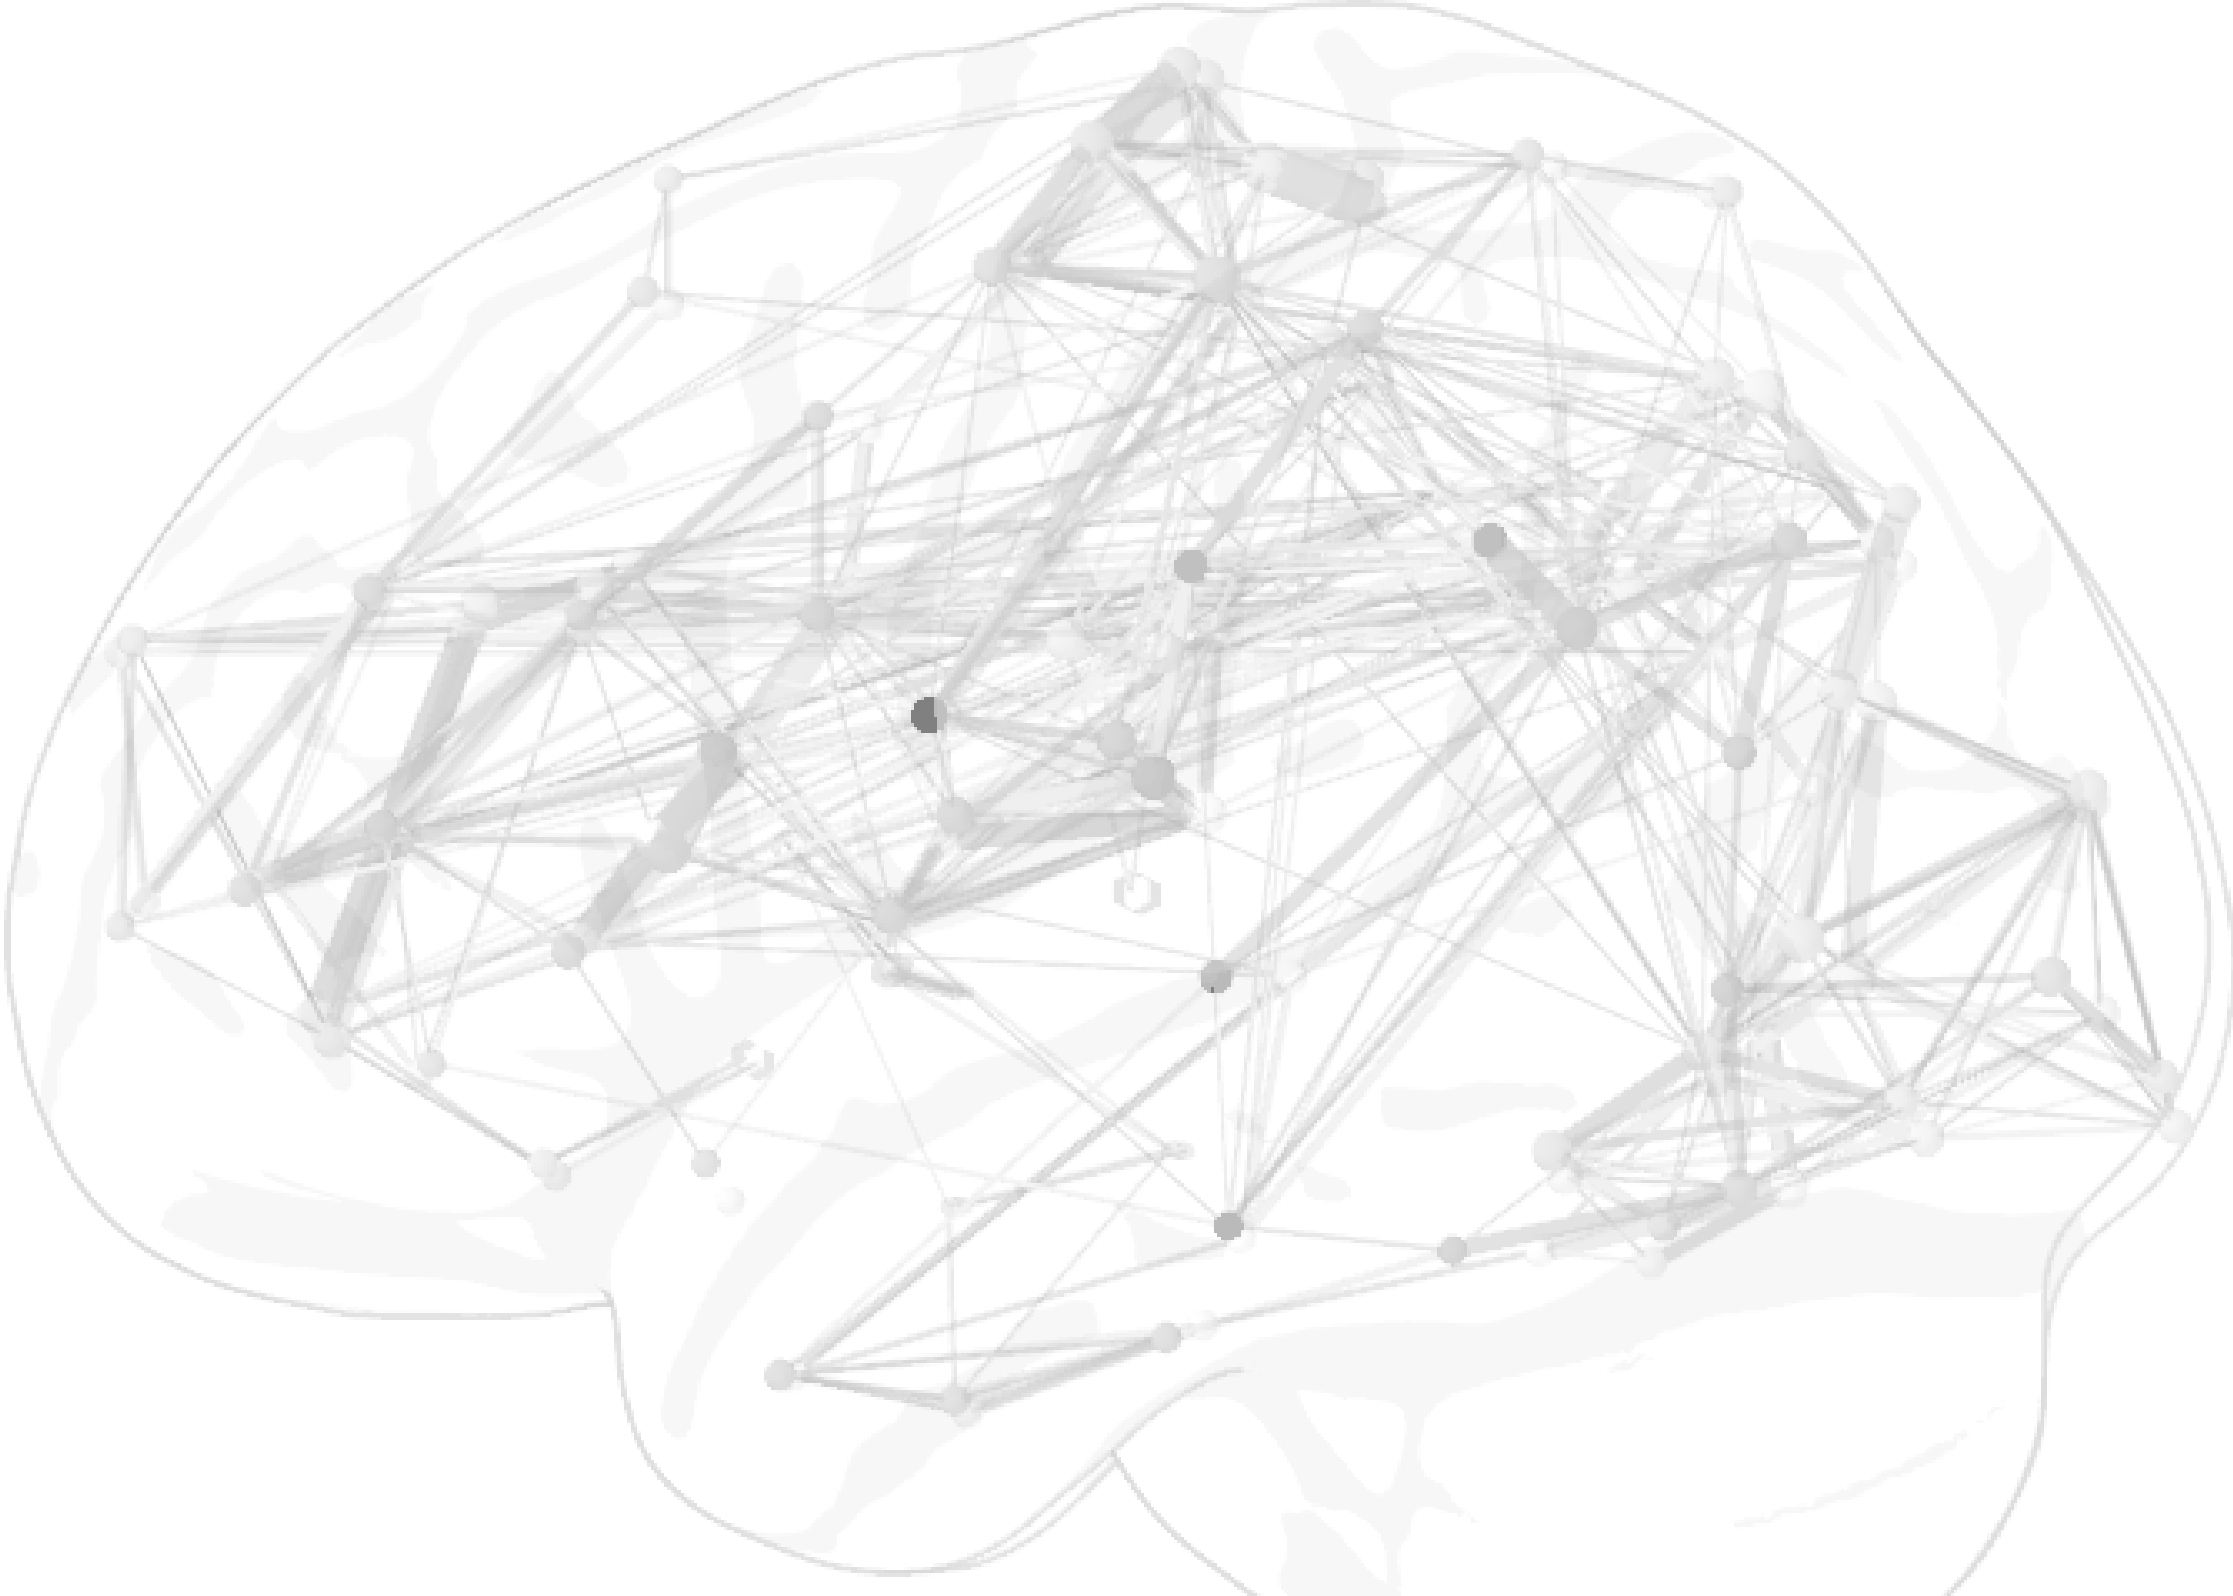
\includegraphics[width=\paperwidth,height=\paperheight]{sfig/bg_conn1}}

\begin{frame}
  \titlepage
\end{frame}
}

\begin{frame}
  \frametitle{fMRI Experiments}
  \centering
  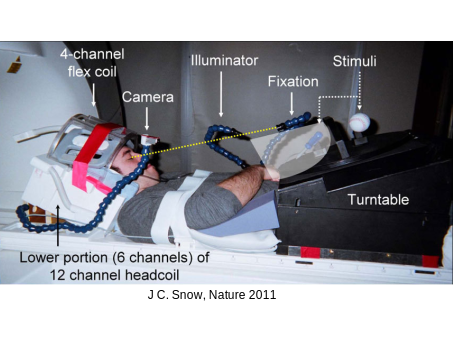
\includegraphics[width=\textwidth]{sfig/fmri_exp}
\end{frame}

\begin{frame}
\frametitle{Clinical Applications of rs-fMRI}
\includegraphics<1>[width=1\textwidth]{sfig/wordcloud}
\includegraphics<2>[width=1\textwidth]{sfig/rsfmri_usage}
\end{frame}

\begin{frame}
\frametitle{Outline}
\tableofcontents[subsectionstyle=show/show/hide]
\end{frame}

\section{Introduction}

% what is fMRI and rs-fMRI, properties. 
%% \subsection{fMRI Images}
\begin{frame}
  \frametitle{Functional MRI Data }
  \begin{columns}[c]
    \begin{column}{5cm}

      \begin{block}{}
        \begin{itemize}
        \item Blood oxygen level dependent (BOLD) indirectly measures neuronal
          activity.
        \item 3D volumes sampled at each time point.
        \item Fast scan, but noisy.
        \item Spatio-temporal dependency.
        \end{itemize}
      \end{block}
      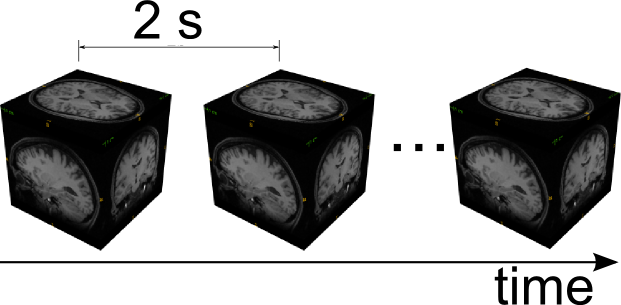
\includegraphics[width=0.8\textwidth]{sfig/4dfmri}
    \end{column}

    \begin{column}{5cm}

      % the fmri file is 53x63
      \includemedia[
        label=vidA,
        addresource=sfig/fmrimovie.swf,
        activate=pageopen,
        width=5.3cm, height=6.3cm,
        flashvars={
          source=sfig/fmrimovie.swf
          &loop=true
        }
      ]{}{sfig/fmrimovie.swf}
    \end{column}
  \end{columns}
  \centering
  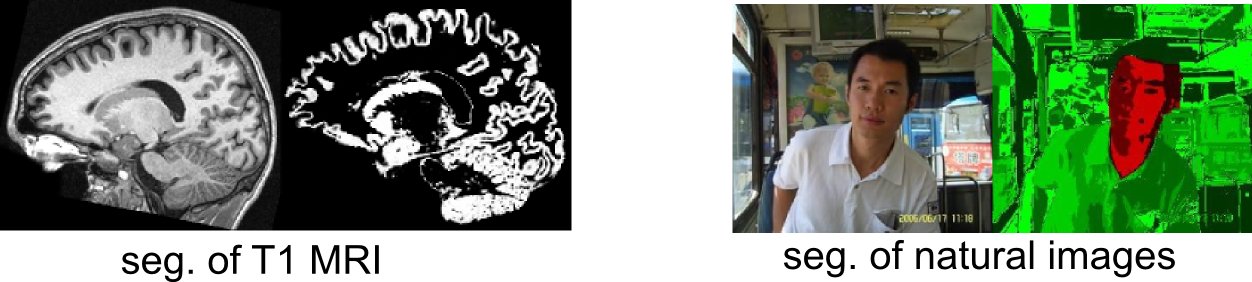
\includegraphics[height=0.2\textheight]{sfig/easy_seg}    

\end{frame}

\begin{frame}
  \frametitle{Task-based v.s. rs-fMRI}
  \begin{columns}[t]
    \begin{column}{5cm}
      \begin{block}{Task-based}
        \begin{itemize}
        \item Experiment stimulus signal.
        \item Subjects undertake cognitive tasks.
        \item Linear regression between stimulus and BOLD.
        \end{itemize}
      \end{block}
      %% \begin{figure}
      %%   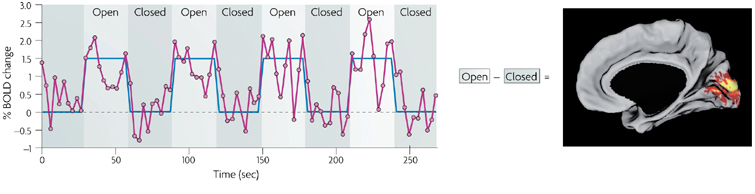
\includegraphics[width=5cm]{sfig/taskfmri}
      %%   \caption{\tiny M. Fox, Nat. Rev., Neuroscience}
      %%   \end{figure}

    \end{column}

    \begin{column}{5cm}
      \begin{block}{Resting-State}
        \begin{itemize}
        \item No experiment paradigm signal.
        \item Subject stays in scanner. Eyes closed/open to a fixation cross.
        \item Correlation between two voxels.
        \end{itemize}
      \end{block}
      %% \begin{figure}
      %%   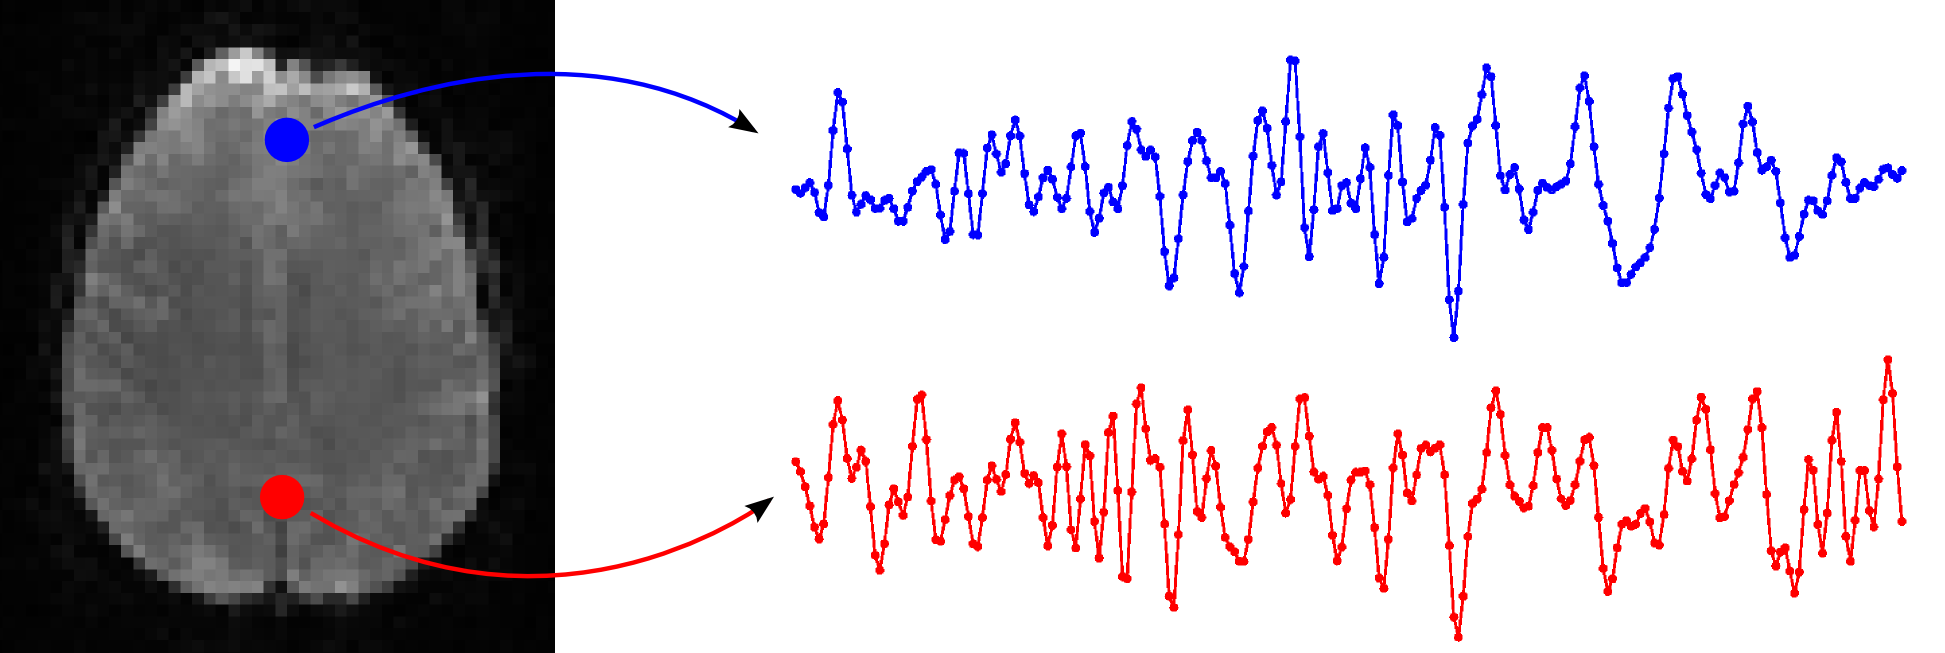
\includegraphics[width=5cm]{sfig/corr}
      %%   \end{figure}
    \end{column}
  \end{columns}
  \vspace{5pt}
  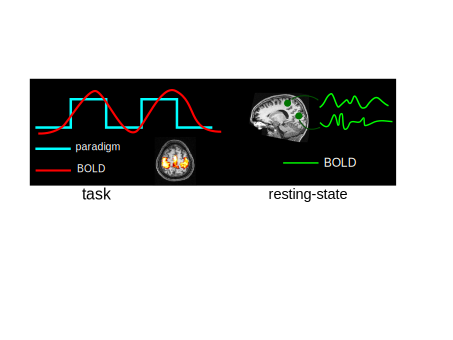
\includegraphics[width=1\textwidth]{sfig/task_rest}
\end{frame}

\subsection{Processing Pipeline}
\begin{frame}
  \frametitle{fMRI Processing Pipeline}
  \begin{figure}
    \includegraphics<1>[width = 1\textwidth]{prep/prep}
    \end{figure}
\end{frame}

% various methods for rs-fMRI and network connectivity.
\subsection{Existing Methods}
\begin{frame}
  \frametitle{Network Analysis Methods}
  \includegraphics<1>[width=1\textwidth]{sfig/allmethods}
\end{frame}

%---------------------------------------------
\subsection{Graphical Model and Markov Random Field}
%% \subsection{Definitions of graphical model and MRF}

% give various graph, undirected and directed. chain, tree, general graph, chain
% graph.
%% \begin{frame}
%%   \frametitle{Graphical Model}
%%   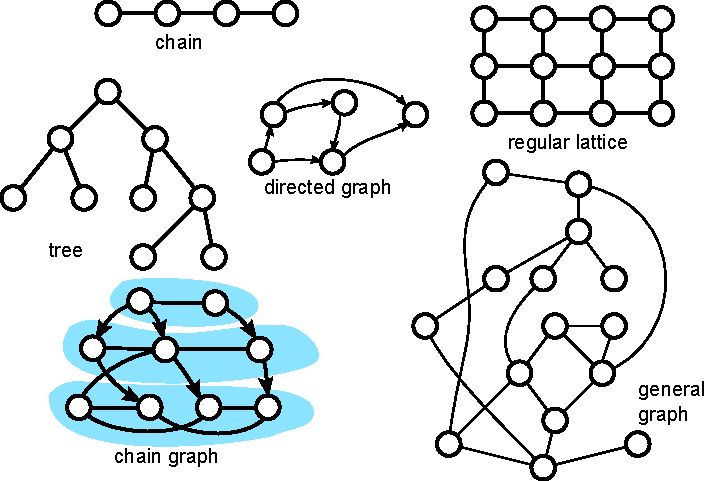
\includegraphics[width = 1\textwidth]{sfig/graphs}
%% \end{frame}

\begin{frame}
\frametitle{Markov Random Field}
\begin{columns}
  \begin{column}{3cm}
    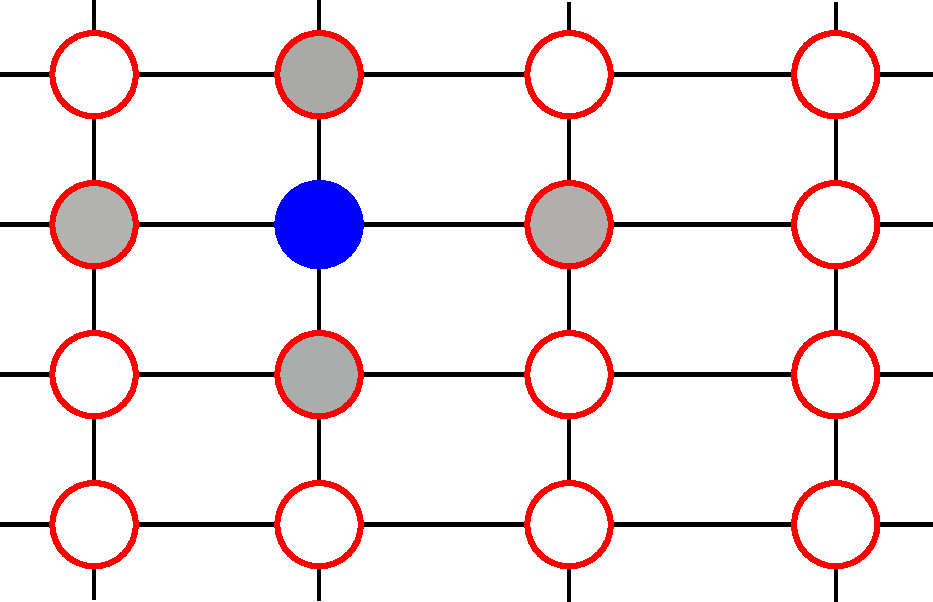
\includegraphics[width=3cm]{sfig/mrf}\\
    \vspace{5pt}
    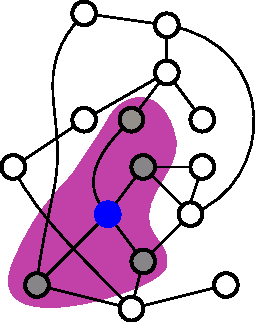
\includegraphics[width=3cm]{sfig/general_mrf}
  \end{column}

  \begin{column}{7cm}

    \begin{definition}
      $\mathcal{G} = (\mathcal{V}, \mathcal{E})$: undirected graph.\\
      $s \in \mathcal{V}$: a node/site in $\mathcal{V}$. \\
      $X = \{x_1, \dots x_N\}$: Set of random variables defined on $\mathcal{G}$.\\
      $\mathcal{N}_s$: Set of nodes neighboring $s$. $(r,s) \in \mathcal{E} \Leftrightarrow  r\in \mathcal{N}_s $.
    \end{definition}

    \begin{definition}
      A \alert{Markov Random Field} (MRF) is a collection of variables $X$ defined on
      graph $\mathcal{G}$ if for all $s \in
      \mathcal{V}$
      \begin{equation*}
        P(s_s | X_{\mathcal{V}-s}) = P(s_s | x_{\mathcal{N}_s})
      \end{equation*}
    \end{definition}
  \end{column}
\end{columns}
\end{frame}


\begin{frame}
\frametitle{MRF and Gibbs Field}

\begin{theorem}[Hammersley-Clifford, 1971]
  $X$ is an MRF on $\mathcal{G}$ if and only if $X$ obeys Gibbs distribution in
  the following form
  \begin{equation*}
    P(X) = \frac{1}{Z}\exp \left( -\frac{1}{T} U(X) \right),
  \end{equation*}

  \begin{equation*}
    U(X) = \sum_{c\in \cC} V_c(X_c).
  \end{equation*}
\end{theorem}

$Vc(X_c) = \beta \sum_{(r,s) \in \cV} \psi(x_r, x_s) $: Ising, Potts model.
\centering
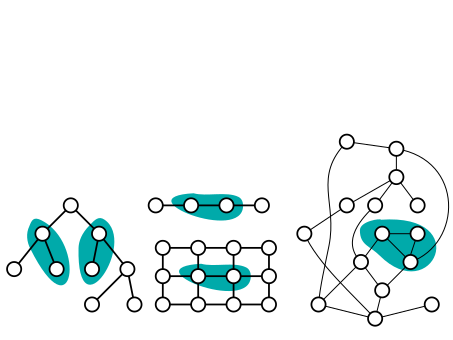
\includegraphics[width = 0.8\textwidth]{sfig/clique_examples}

%% Gibbs distribution gives a global property that can be used as a prior
%% distribution.
\end{frame}

%----------------------------------------------------------
\begin{frame}
  \frametitle{Hidden Markov Model: A Generative Model}
  \begin{columns}
    \begin{column}{0.5\textwidth}
      \begin{block}{}
        \begin{itemize}
          \item $X$ is defined on MRF. 
          \item $Y$ is assumed to be generated from $X$.
          \item Inverse problem: Given Y, estimate X.
          %% \item Different from structure learning problem. 
        \end{itemize}
      \end{block}
    \end{column}

    \begin{column}{0.5\textwidth}
      \centering
      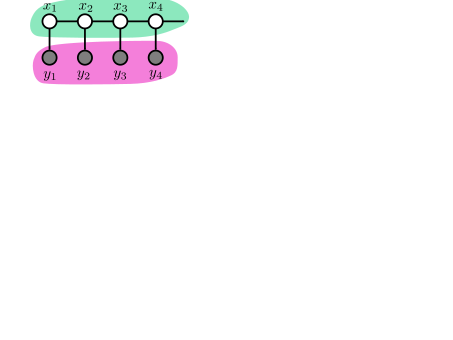
\includegraphics[width = 0.7\textwidth]{sfig/hmm_chain}\\
      \vspace{5mm}
      \includegraphics[width=0.7\textwidth]{sfig/hmm}      
    \end{column}
  \end{columns}

  \begin{columns}
    \begin{column}{0.5\textwidth}
      \centering
      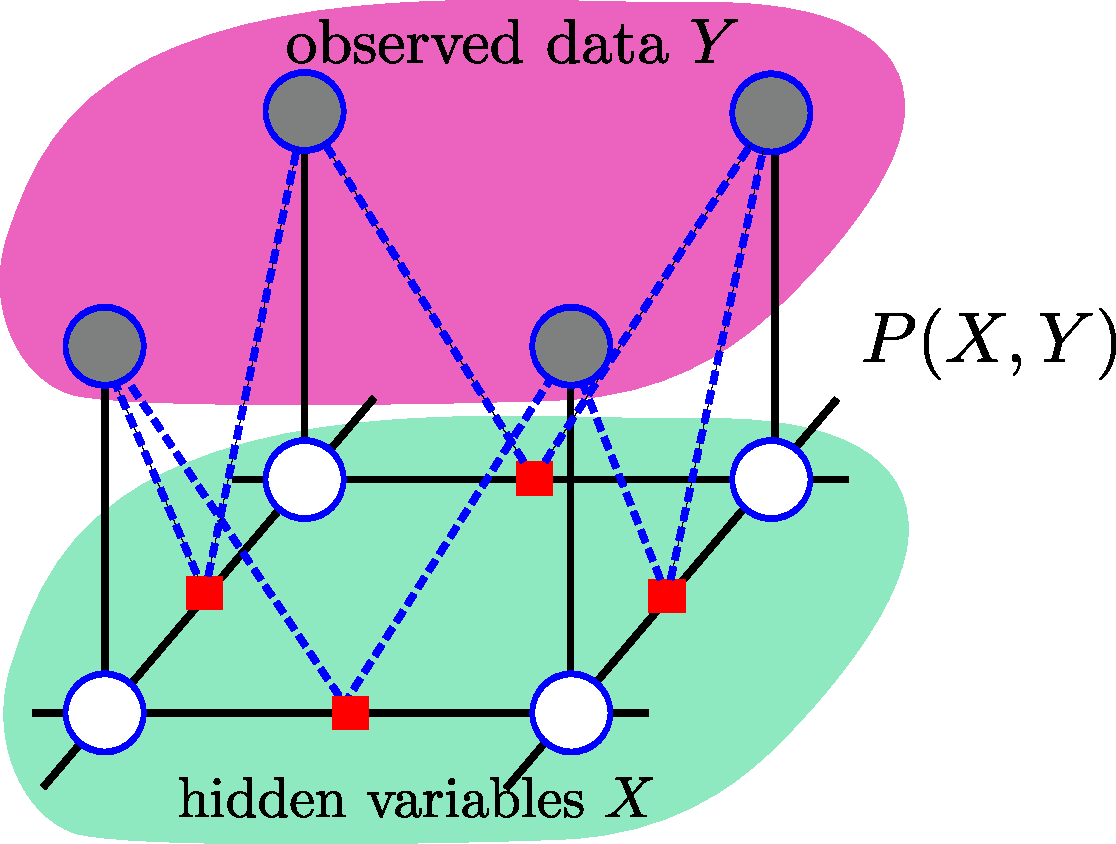
\includegraphics[width = 0.7\textwidth]{sfig/crf}
      \end{column}
    \begin{column}{0.5\textwidth}
      \begin{block}{}

        Other forms exist: conditional random field, but no Bayesian
        interpretation.
      \end{block}
      \end{column}
    \end{columns}

\end{frame}

\section{Pairwise Connectivity with Six Dimensional MRF}

\begin{frame}<beamer>
  \frametitle{Outline for section \thesection}
  \tableofcontents[currentsection, sectionstyle=show/hide, subsectionstyle=show/show/hide]
\end{frame}

\subsection{Problem Statement}
\begin{frame}
  \frametitle{Pairwise Connectivity With Spatial Coherence}
  \begin{columns}
    \begin{column}{0.5\textwidth}
      \begin{block}{The Goal}
        \begin{itemize}
        \item The connectivity between each pair of voxels in single subject
          rs-fMRI.
        %% \item No Seed region needed.
        \item Spatial regularization by MRF, without changing signals. 
        \item Learn the strength of the smoothness from the data.
        \end{itemize}
      \end{block}
      \end{column}
    \begin{column}{0.5\textwidth}
      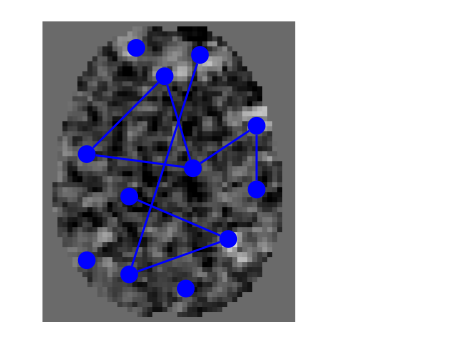
\includegraphics[width=0.9\textwidth]{sfig/pairwise_conn}
    \end{column}
  \end{columns}
\end{frame}

\subsection{A Six Dimensional MRF model}
\begin{frame}
\frametitle{Pairwise Connectivity With Spatial Coherence: the Model}
  \begin{columns}
    \begin{column}{0.45\textwidth}
      \begin{block}{Model Definition}
        \begin{itemize}
        \item MRF defined on 6D graph.
        \item Pairwise connectivity variable $X\in \{0, 1\}^N$, sample correlation $Y$. 
        %% \item Add an edge $(x_{ij}, x_{st})$ if any voxels between $i,j$ and
        %%   $s,t$ are neighbors.
        \item $(x_{ij}, x_{ik}) \in \cE \Leftrightarrow j\in \cN(k)$.
          \item $ P(F(y_{ij}) |x_{ij}) \sim \mathcal{N}(\mu, \sigma^2)$.
        %% \item Variational Bayesian inference for  $X$.
        \end{itemize}
      \end{block}
    \end{column}
    \begin{column}{0.55\textwidth}
      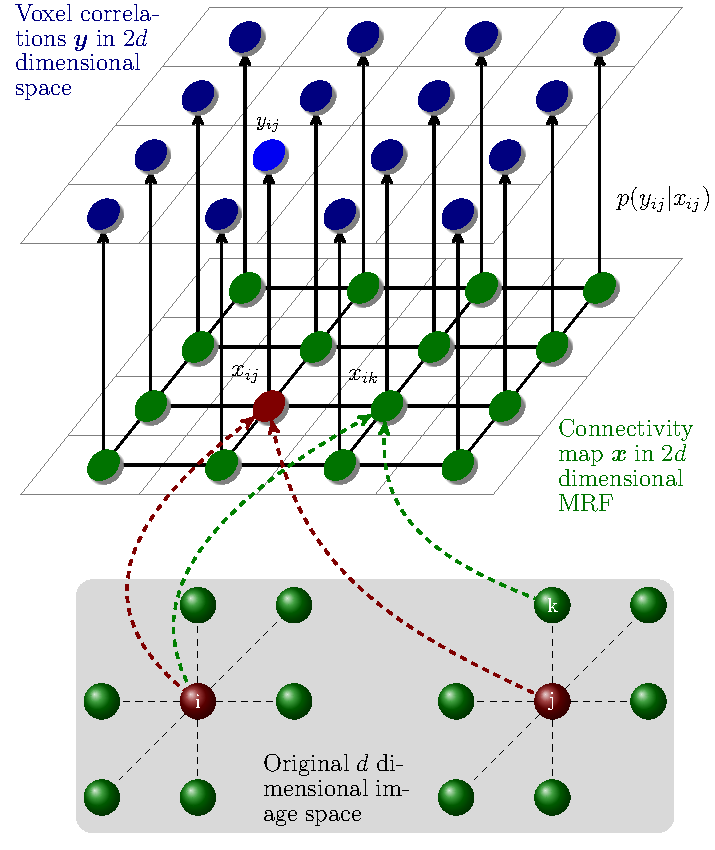
\includegraphics[width=\textwidth]{sfig/6dmrf}
    \end{column}
    \end{columns}
\end{frame}


\subsection{Statistical Inference}
\begin{frame}
  \frametitle{Statistical Inference}

  \begin{columns}
    \begin{column}{0.65\textwidth}
      \begin{block}{Questions}
        \begin{itemize}
        \item Given $x_{-s}$ and $Y$, what is $P(x_s)$. 
        \item $x_s = \argmax P(X|Y)$
        \item \alert{$X^* = \argmax P(X | Y)$.}
        \end{itemize}
      \end{block}

      \begin{block}{Algorithms}
        \begin{itemize}
        \item Exact solutions for simple graphs (trees, chains): sum-product,
          max-sum, belief propagation.
        \item No exact solution for general graphs. 
        \end{itemize}
      \end{block}
      \includegraphics<1>[width=0.8\textwidth]{sfig/chaintree}
      \includegraphics<2>[width=0.8\textwidth]{sfig/chaintree_check}
    \end{column}

    \begin{column}{0.35\textwidth}
      \includegraphics<1>[height=0.9\textheight]{sfig/generalgraphs}
      \includegraphics<2>[height=0.9\textheight]{sfig/generalgraphs_check}
    \end{column}

    \end{columns}
\end{frame}

\begin{frame}
  \frametitle{Approximate Inference}
  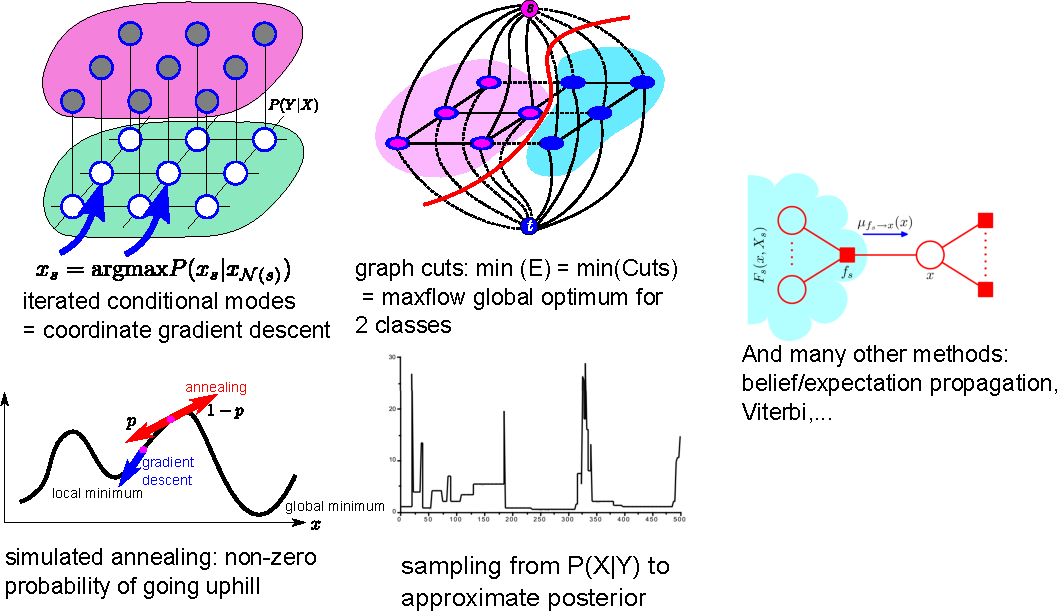
\includegraphics[width=\textwidth]{sfig/appinference}
\end{frame}

\begin{frame}
  \frametitle{Variational Inference}
  \begin{block}{}
    \begin{itemize}
    \item Assuming $Q(X) = \prod_s q_s(x_s)$.
    \item Search $Q(x)$ in a smaller space.
    \item $\log Q_s(x_s) = E_{r\neq s} [ \log P(X, Y)] + \textrm{const}$
    \end{itemize}
  \end{block}
  \vspace{10pt}
  \centering
  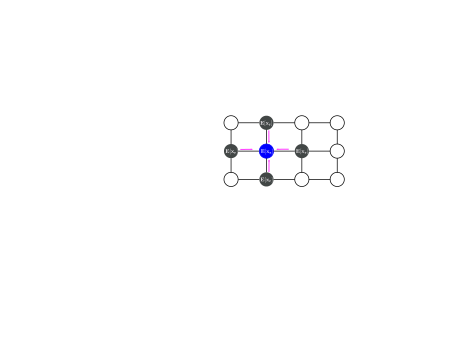
\includegraphics[width=0.5\textwidth]{sfig/variational_inf}
\end{frame}

%% We first construct a synthetic data set consisting of a 100  1
%% 1-D image, with each pixel a 300-point time course signal. The time course was
%% constructed with a baseline DC signal of 800, plus additive Gaussian noise of
%% variance 50. We then added a sine wave signal of frequency 0.2 and amplitude
%% 20 to two distant regions of the image.

\subsection{Experiments on Synthetic and Real Data}
\begin{frame}
  \frametitle{Experiments}
  \begin{columns}
    \begin{column}{0.6\textwidth}

      \uncover<1,2>{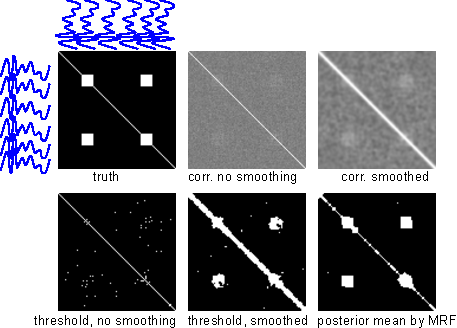
\includegraphics[width=1\textwidth]{sfig/m1_syn}}
    \end{column}
    \begin{column}{0.4\textwidth}
      \uncover<1,2> {
        \begin{block}{Simulated data}
          \begin{itemize}
          \item Construct 1D image. Connected voxels are added with sine wave
            signal.
          \item Spatial smoothing improves results, but increased false positive.

          \end{itemize}
        \end{block}
      }
    \end{column}
  \end{columns}
  \vspace{5pt}
  \begin{columns}
    \begin{column}{0.4\textwidth}
      \uncover<2> {
        \begin{block}{Real data}
          \begin{itemize}
          \item connectivity between a voxel in PCC and current slice.
          \item Detecting PCC-MPFC links in default mode network.
          \end{itemize}
        \end{block}
      }

    \end{column}
    \begin{column}{0.6\textwidth}
      \uncover<2> {
        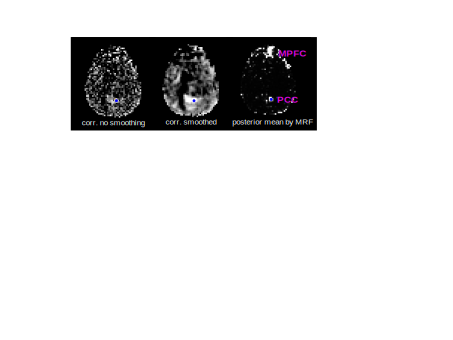
\includegraphics[width=1.0\textwidth]{sfig/m1_real}
      }
    \end{column}
  \end{columns}
\end{frame}

\section{Consistent, Spatially Coherent Multiple Functional Networks}

\begin{frame}<beamer>
  \frametitle{Outline for section \thesection}
  \tableofcontents[currentsection, sectionstyle=show/hide, subsectionstyle=show/show/hide]
\end{frame}


\subsection{Problem Statement}
\begin{frame}
\frametitle{Consistent, Spatially Coherent Multiple Functional
  Networks}
\begin{block}{The Goal}
  \begin{itemize}
  \item Partition the brain into multiple functional networks.
  \item Spatial coherence is respected.
  \item Parameter estimation.
  \end{itemize}
\end{block}
\vspace{10pt}
\begin{figure}
  \centering
  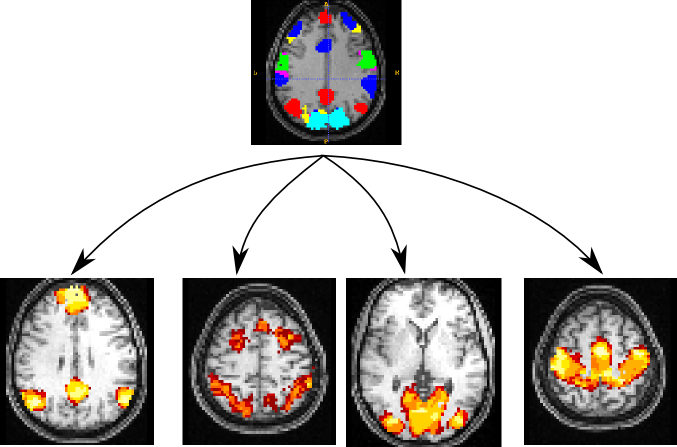
\includegraphics[width=0.7\textwidth]{sfig/myseg}
\end{figure}
\end{frame}

\subsection{A MAP framework with MRF prior}
\begin{frame}
\frametitle{MRF and vMF Models}

\begin{columns}
  \begin{column}{0.6\textwidth}
    \centering
    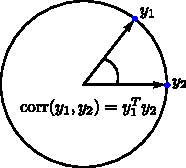
\includegraphics[width=0.6\textwidth]{sfig/vmf}

      \begin{block}{Model}
        \begin{itemize}
        \item  $P(X) = (1/Z) \exp \left ( -\beta \sum_{(r,s)\in \mathcal{E}} \psi(x_s, x_r)\right )$.
          \item $x_s \in \{1, \dots, L\}$
        \item  $P(y_s | x_s) = C_p(\kappa_l) \exp (\kappa_l \mu_l^{\top} y_s)$, \\
          $y_s \in S^{p-1}$ (von Mises-Fisher distribution).
        \item Solve $P(X | Y) \propto P(X) \cdot P(Y|X) $
        \end{itemize}
      \end{block}
      \end{column}

  \begin{column}{0.4\textwidth}
    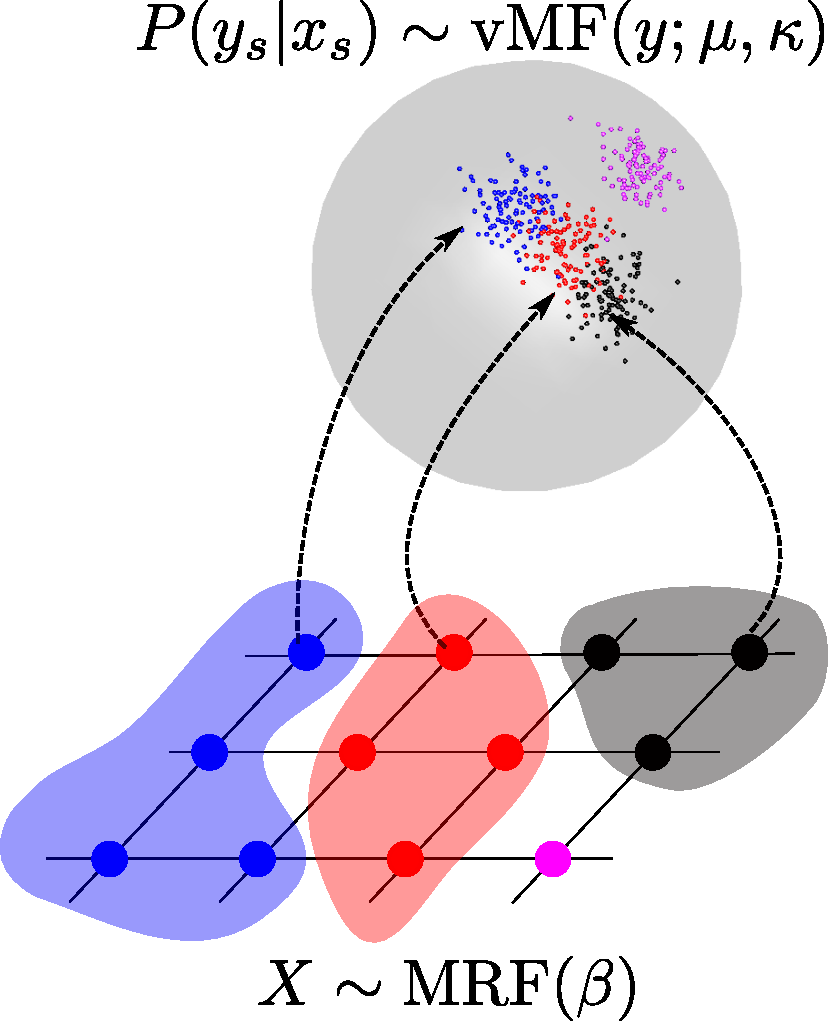
\includegraphics[width=1\textwidth]{sfig/genevmf}
  \end{column}
\end{columns}
\end{frame}

\subsection{MCEM for Statistical Inference}
\begin{frame}
\frametitle{Statistical Inference by MCEM}

\begin{columns}[t]
  \begin{column}{0.6\textwidth}
    \uncover<1,2,3>{
      \begin{block}{Expectation Maximization}
        $Q(\theta) = \mathbb{E}_{X|Y} [\log P(X,Y;\theta)]$
      \end{block}
    }

    \uncover<2,3> {
      \begin{block}{Pseudo Likelihood}
        $ \log P(X^m; \theta) \approx \sum_{s\in \mathcal{V}} \log P(x_s | x_{\mathcal{N}_s};\theta)$
      \end{block}
    }
    \only<3> {
      \begin{block}{Parameter Estimation}
        $\hat \mu_l = \parallel R_l\parallel, R_l = \sum_{s \in \cV_l}^{} y_s $ \\
        $\hat \kappa_l \approx (pR_l - R^3) / (1 - R^2) $\\
        $\hat \beta = \argmax_\beta \log P(X; \theta)$ by Newton's method. 
      \end{block}
    }

    \end{column}

  \begin{column}{0.4\textwidth}

    \only<1,2,3>
    {
      \begin{block}{Monte Carlo Expectation Maximization (MCEM)}
        \begin{align*}
          & \mathbb{E}_{X|Y} [\log P(X,Y;\theta)] \\
          &\approx \frac{1}{M}\sum_m \log P(X^m, Y; \theta)
        \end{align*}
        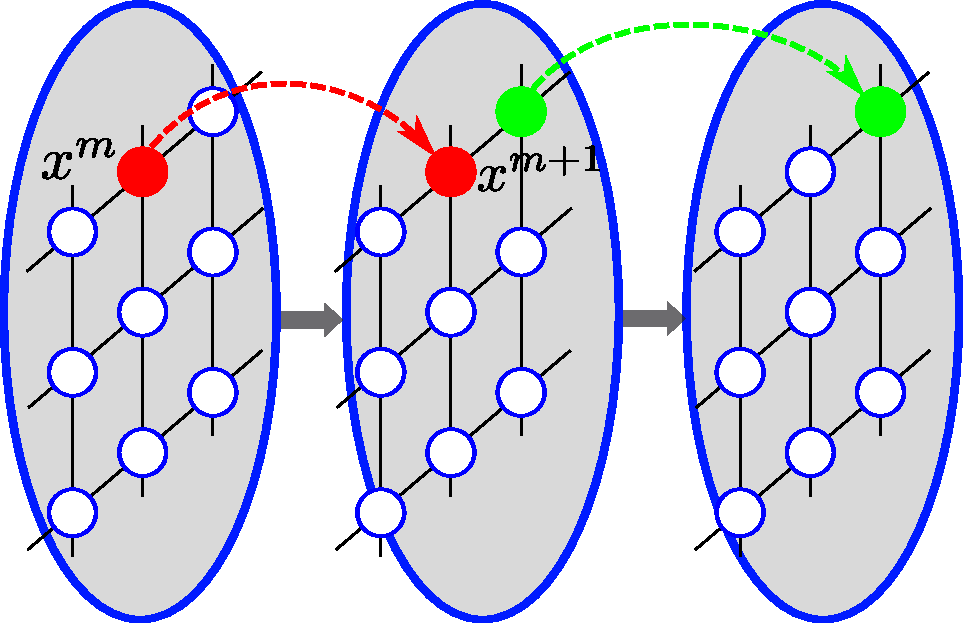
\includegraphics[width=1\textwidth]{sfig/imagechain_mcmc}
      \end{block}
    }
  \end{column}
\end{columns}
\end{frame}

\begin{frame}
  \frametitle{Simulation of Ising and Potts Models}
    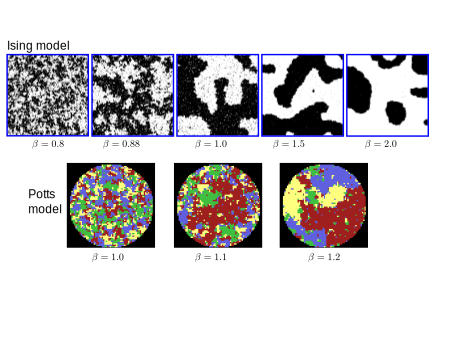
\includegraphics[width=1\textwidth]{sfig/simulations}\\
  % beta = 1.0, 1.1 and 1.2, and scan 500 burn-ins. 
  \centering
    \includemedia[
      %% label=vidB,
      addresource=sfig/gibbs_samples.swf,
      activate=pageopen,
      width=3cm, height=3cm,
      flashvars={
        source=sfig/gibbs_samples.swf
        &loop=true
      }
    ]{}{sfig/gibbs_samples.swf}
% beta = 1.1, burn-in = 300 for the gibbs movie
\end{frame}

\subsection{Experiments on Synthetic Data and Real Data}
\begin{frame}
  \frametitle{Experiments}
  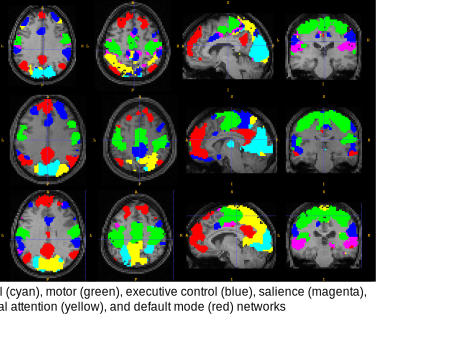
\includegraphics[width=1\textwidth]{sfig/m2_real}
\end{frame}

\section{Consistent Group Analysis by Hierarchical MRF}

\begin{frame}<beamer>
  \frametitle{Outline for section \thesection}
  \tableofcontents[currentsection, sectionstyle=show/hide, subsectionstyle=show/show/hide]

\end{frame}

\subsection{A Two-Way Unified Model}
\begin{frame}
  \frametitle{ Hierarchical Model: a Better Approach}
  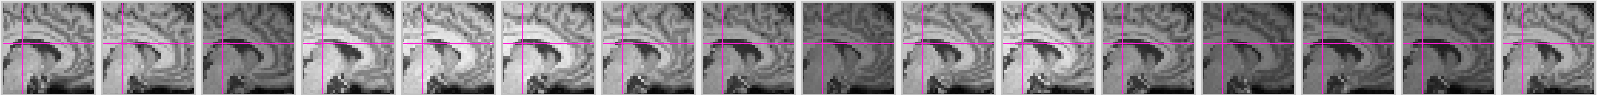
\includegraphics[width=\textwidth]{sfig/allsubs} \\
  \vspace{3pt}
  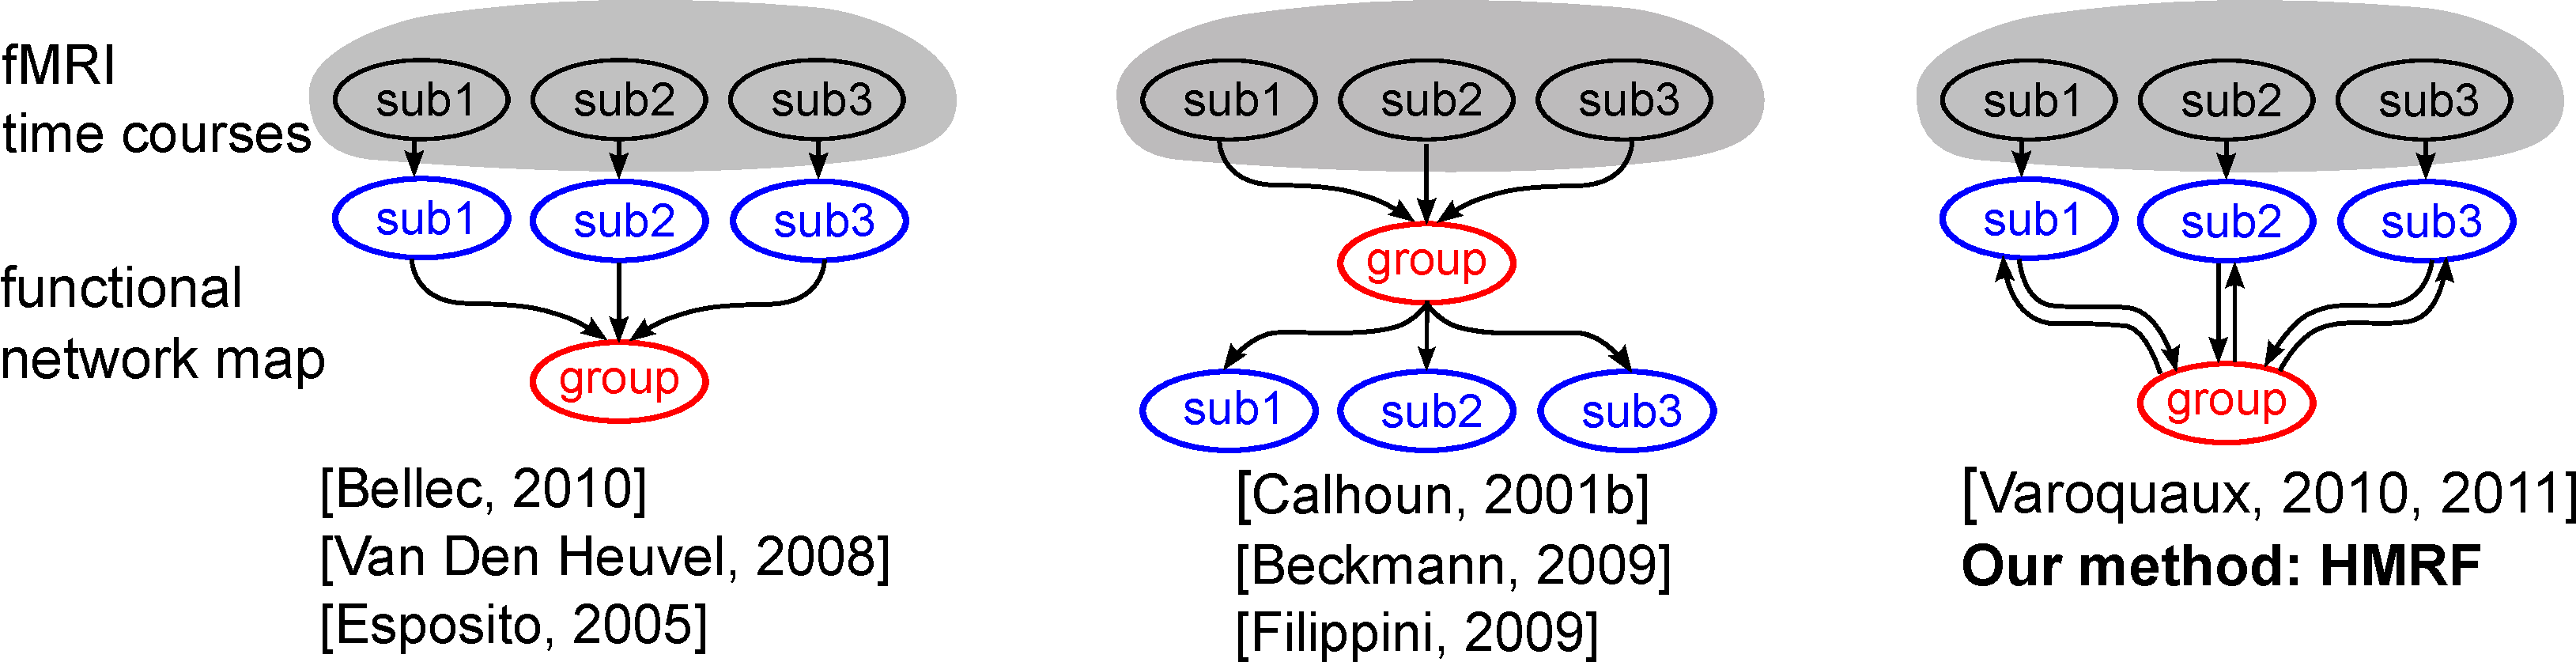
\includegraphics[width=\textwidth]{sfig/bidirections}\\
  \vspace{3pt}
  \begin{columns}
    \begin{column}{0.4\textwidth}
      \begin{block}{Existing Methods}
        \begin{itemize}
        \item Bottom-up or top-down. 
        \item Subject is estimated independently. 
        %% \item Lose fine structures due to spatial smoothing.
        \item Estimation is one way. 
        \end{itemize}
      \end{block}
    \end{column}
  
    \begin{column}{0.6\textwidth}
      \begin{block}{We Propose}
        \begin{itemize}

        \item A hierarchical structure including group and subject. 
        %% \item Each subject has its own variance. 
        %% \item MRF prior for within- and between-subject constraints.
        \item Jointly estimate both levels iteratively.
        \item Bayesian framework. Data driven. Parameter estimation.
        \end{itemize}
      \end{block}
    \end{column}
  \end{columns}
\end{frame}

\subsection{An Extended MRF}
\begin{frame}
  \frametitle{Joint Estimation with MRF}
  \begin{block}{Build a graph}
    \begin{itemize}
    \item within-subject piecewise constant constraints.
    \item Between-subject (between-level) dependency. 
    \end{itemize}
  \end{block}
  \vspace{10pt}
  \centering
  \includegraphics<1>[width=0.7\textwidth]{sfig/hier3a}
  %% \includegraphics<2>[width=0.7\textwidth]{sfig/abstract_layer}
\end{frame}

\begin{frame}
  \frametitle{A Graphical View of the Hierarchical Model}
  \includegraphics<1>[width=1\textwidth]{sfig/grp1}
  \includegraphics<2>[width=1\textwidth]{sfig/grp2}

  \begin{block}{Likelihood}
    $P(y_s | x_s) \sim vMF(\mu, \kappa)$
  \end{block}
\end{frame}

\subsection{Gibbs Sampling for Inference}
\begin{frame}
  \frametitle{Bayesian Inference: Gibbs Sampling}
  \begin{block}{}
    \begin{itemize}
      \item Monte Carlo Sampling used to approximate $\mathbb{E}_{X|Y} [\log
        P(X,Y;\theta)]$.
        \item Gibbs sampling also in a multi-level fashion.
    \end{itemize}
    \end{block}

  \begin{columns}
    \begin{column}{0.5\textwidth}
      \begin{figure}
        \includegraphics[width=1\textwidth]{sfig/hiergibbs2}
        %% \caption{Sampling schedule is also hierarchical.}
        \end{figure}
      \end{column}
    \begin{column}{0.5\textwidth}
      \begin{figure}
        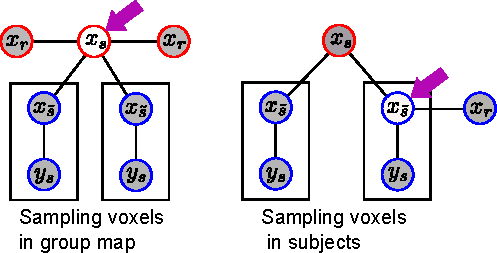
\includegraphics[width=1\textwidth]{sfig/voxelgibbs}
        %% \caption{At voxel level, sample each data point given other data points within and between subject. }
        \end{figure}
    \end{column}
\end{columns}


\end{frame}

\subsection{Experiments on Synthetic Data}
\begin{frame}
  \frametitle{Synthetic Data: Estimation}
  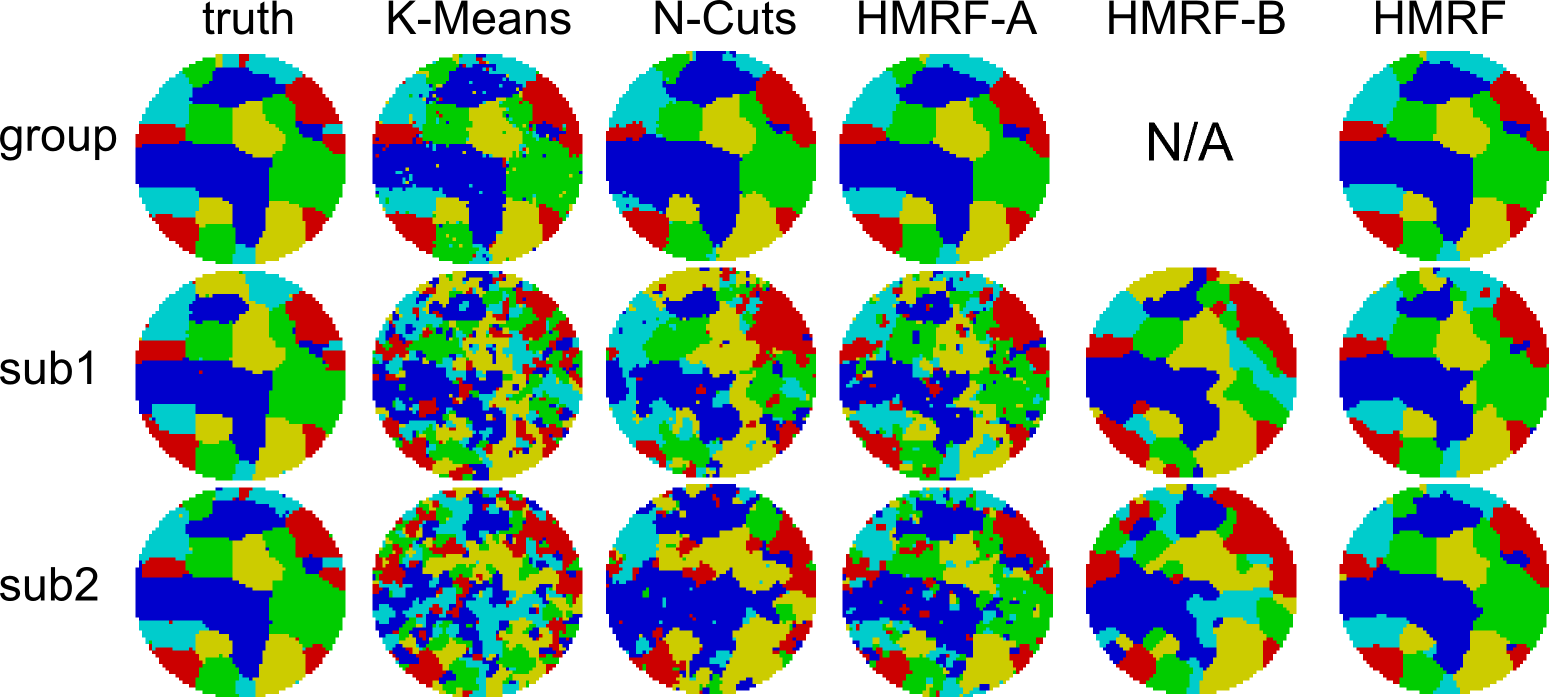
\includegraphics[width = 1\textwidth]{sfig/allmaps}
\end{frame}



\subsection{Cross-Session Consistency}
\begin{frame}
  \frametitle{Cross-Session consistency}
  \centering
  \uncover<1,2> {
    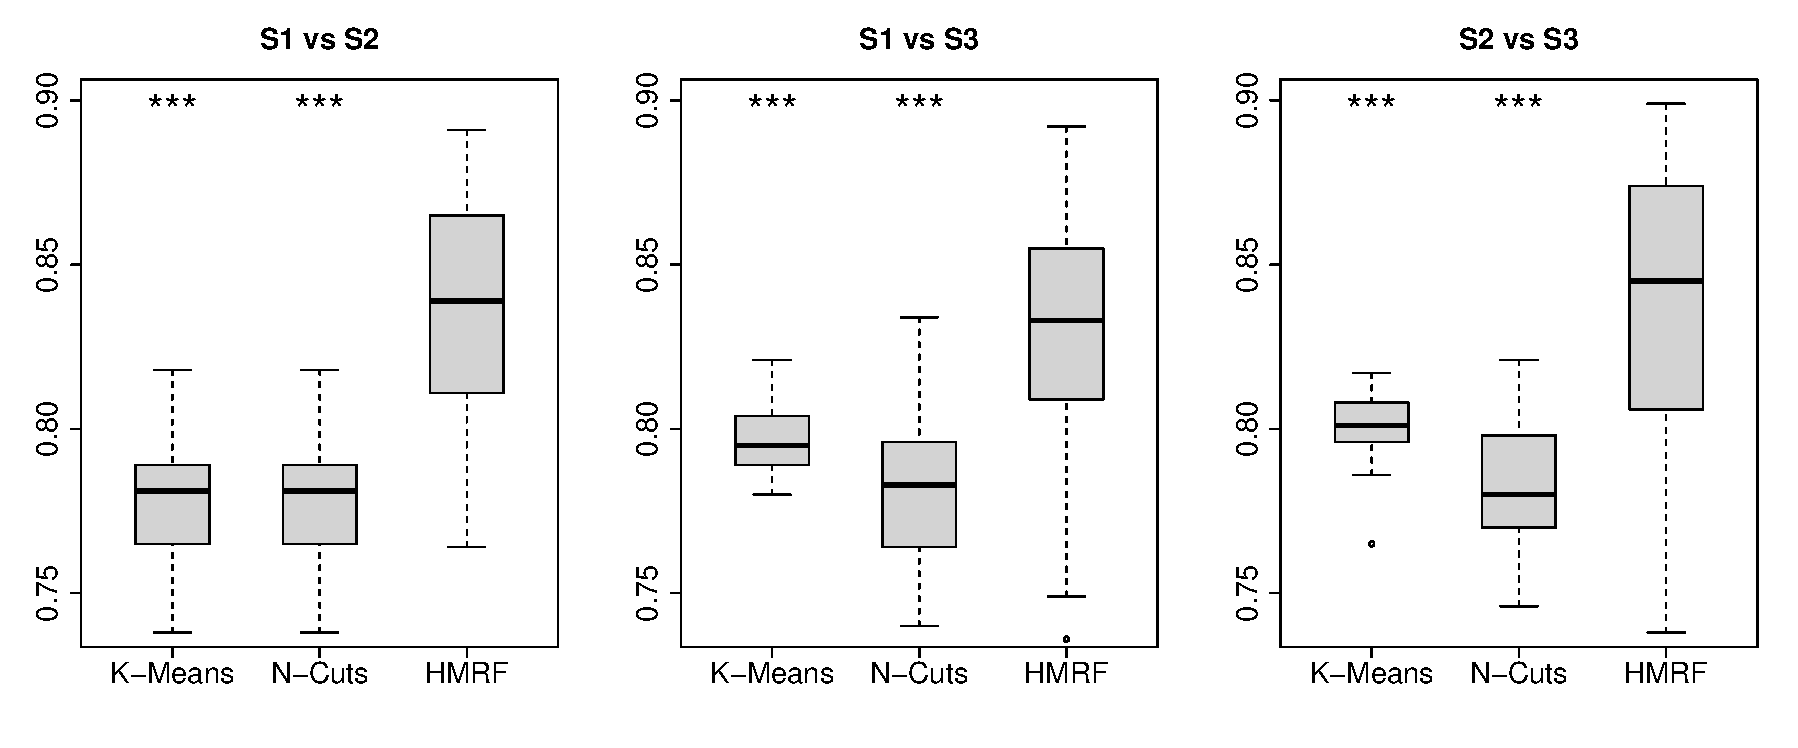
\includegraphics[width = 1\textwidth]{sfig/boxplot}\\
  }
  \uncover<2> {
    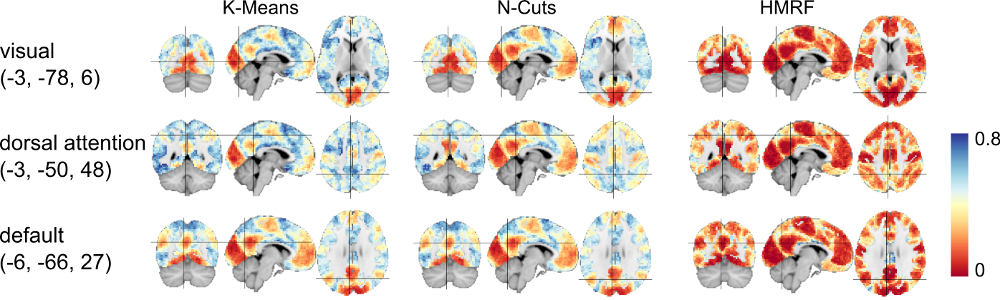
\includegraphics[width = 1\textwidth]{sfig/012variance}
  }
\end{frame}

\subsection{Variability in Bootstrapping}
\begin{frame}
\frametitle{Bootstrapping: Group Mean Maps}
\centering
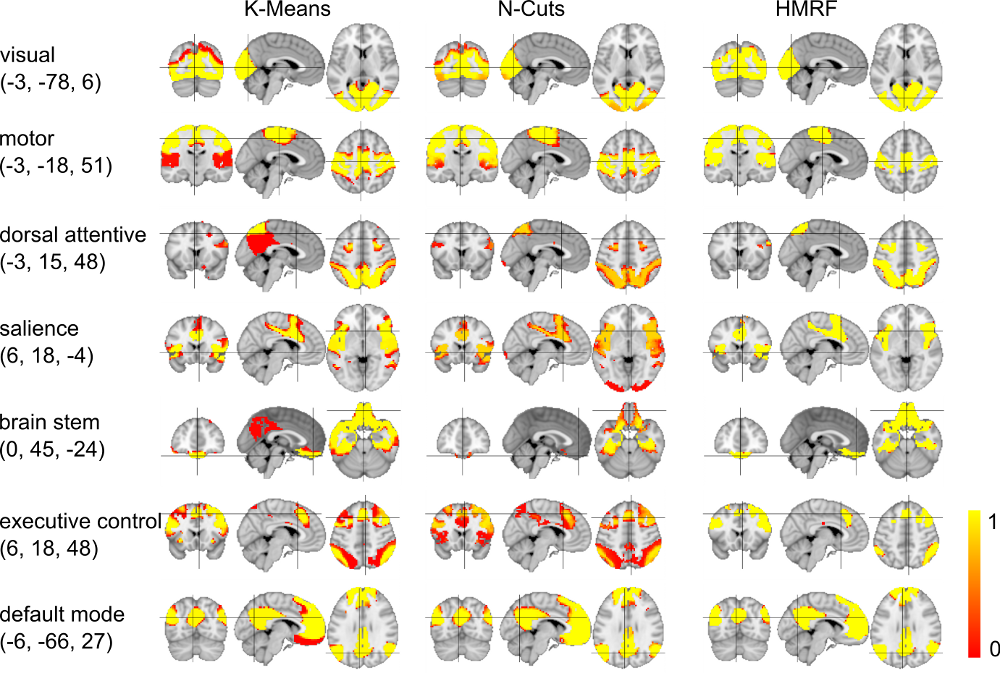
\includegraphics[width = 1\textwidth]{sfig/grp_mean}
\end{frame}

%% \begin{frame}
%% \frametitle{Bootstrapping: Group Variance Maps}
%% \centering
%% 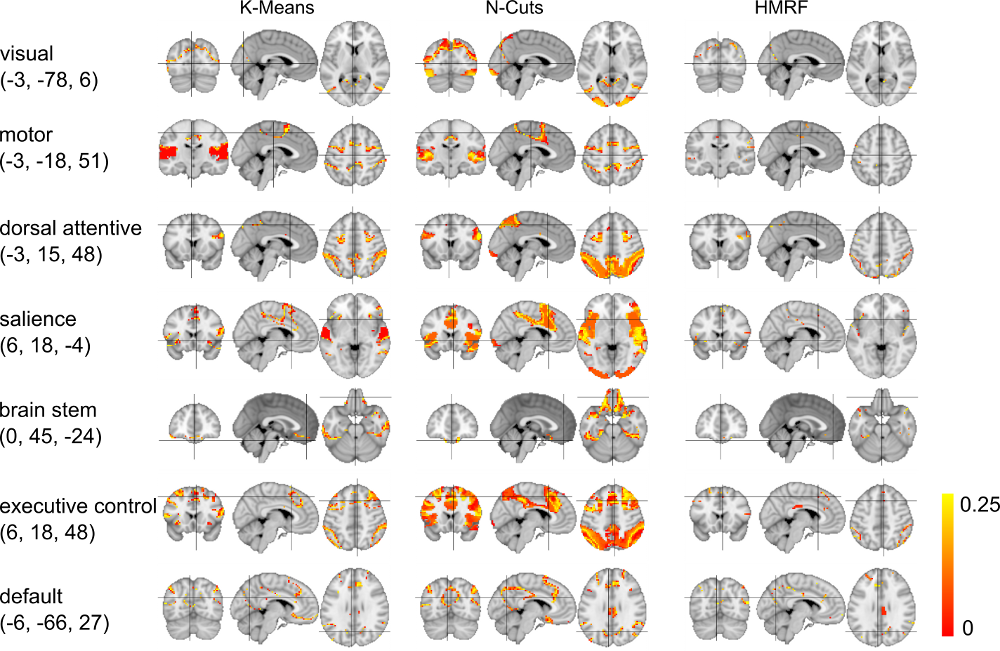
\includegraphics[width = 1\textwidth]{sfig/grp_var}
%% \end{frame}

\begin{frame}
\frametitle{Bootstrapping: Subject Mean Maps}
\centering
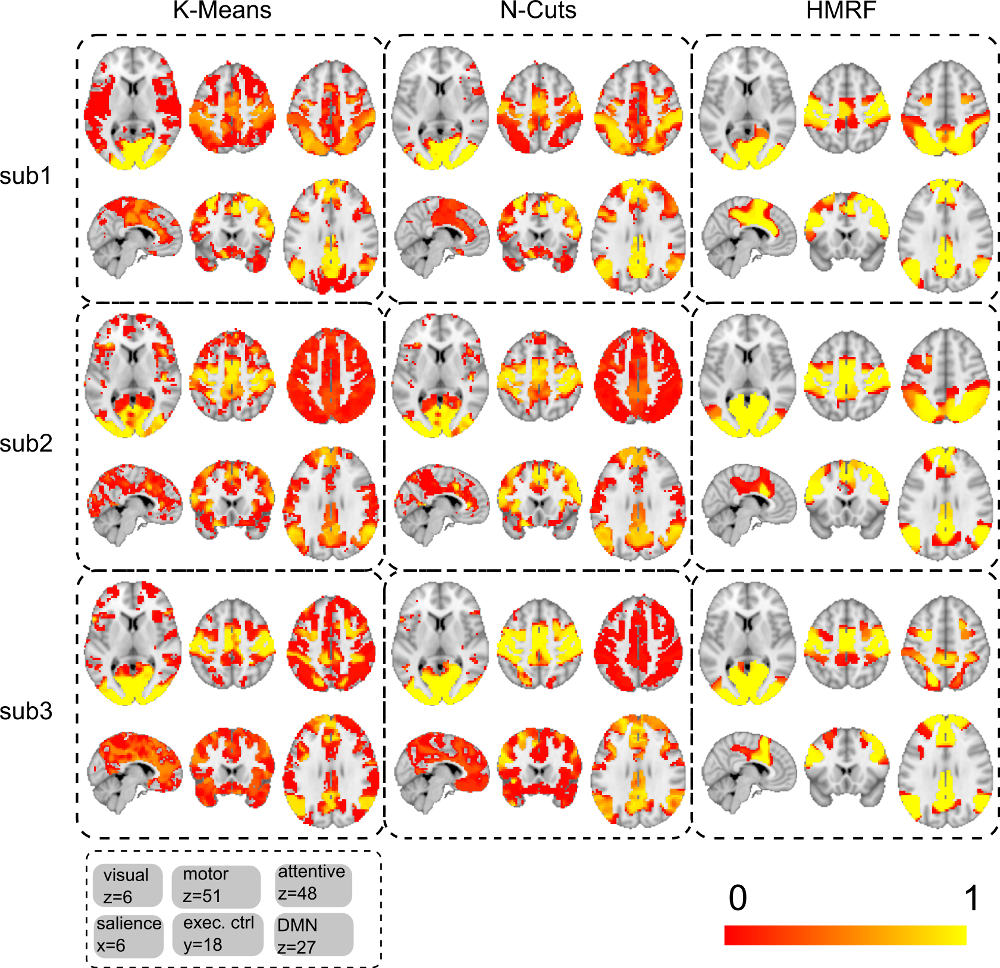
\includegraphics[width = 0.7\textwidth]{sfig/submean}
\end{frame}



\section{Traumatic Brain Injury Image Segmentation with Active Learning}

\begin{frame}<beamer>
  \frametitle{Outline for section \thesection}
  \tableofcontents[currentsection, sectionstyle=show/hide, subsectionstyle=show/show/hide]
\end{frame}

\subsection{The Problem}
\begin{frame}
  \frametitle{Traumatic Brain Injury Image Segmentation with Active Learning: Motivation}
  \begin{block}{}
    \begin{itemize}
      \item Multi-modality, longitudinal, complex patterns. 
      \item Existing methods: high false-positive/negative, 2D, single object.
      \item A slight user involvement significantly improves result.
      \item Computer active, user passive (less burden).
    \end{itemize}
  \end{block}
  \centering
  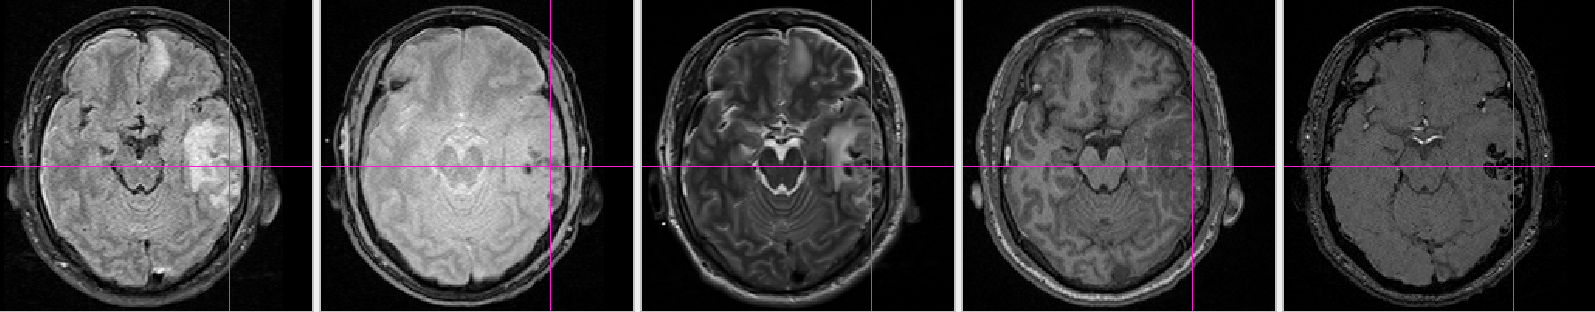
\includegraphics[width=0.75\textwidth]{actlearn_fig/allchannels}\\
  \vspace{2pt}
  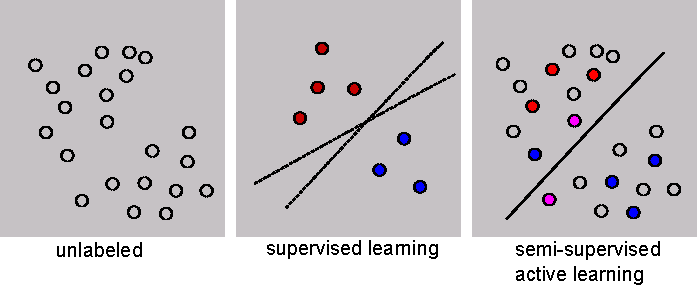
\includegraphics[width=0.8\textwidth]{actlearn_fig/activelearn}
\end{frame}

\subsection{The Flowchart}
\begin{frame}
  \frametitle{An Active Learning Framework}
  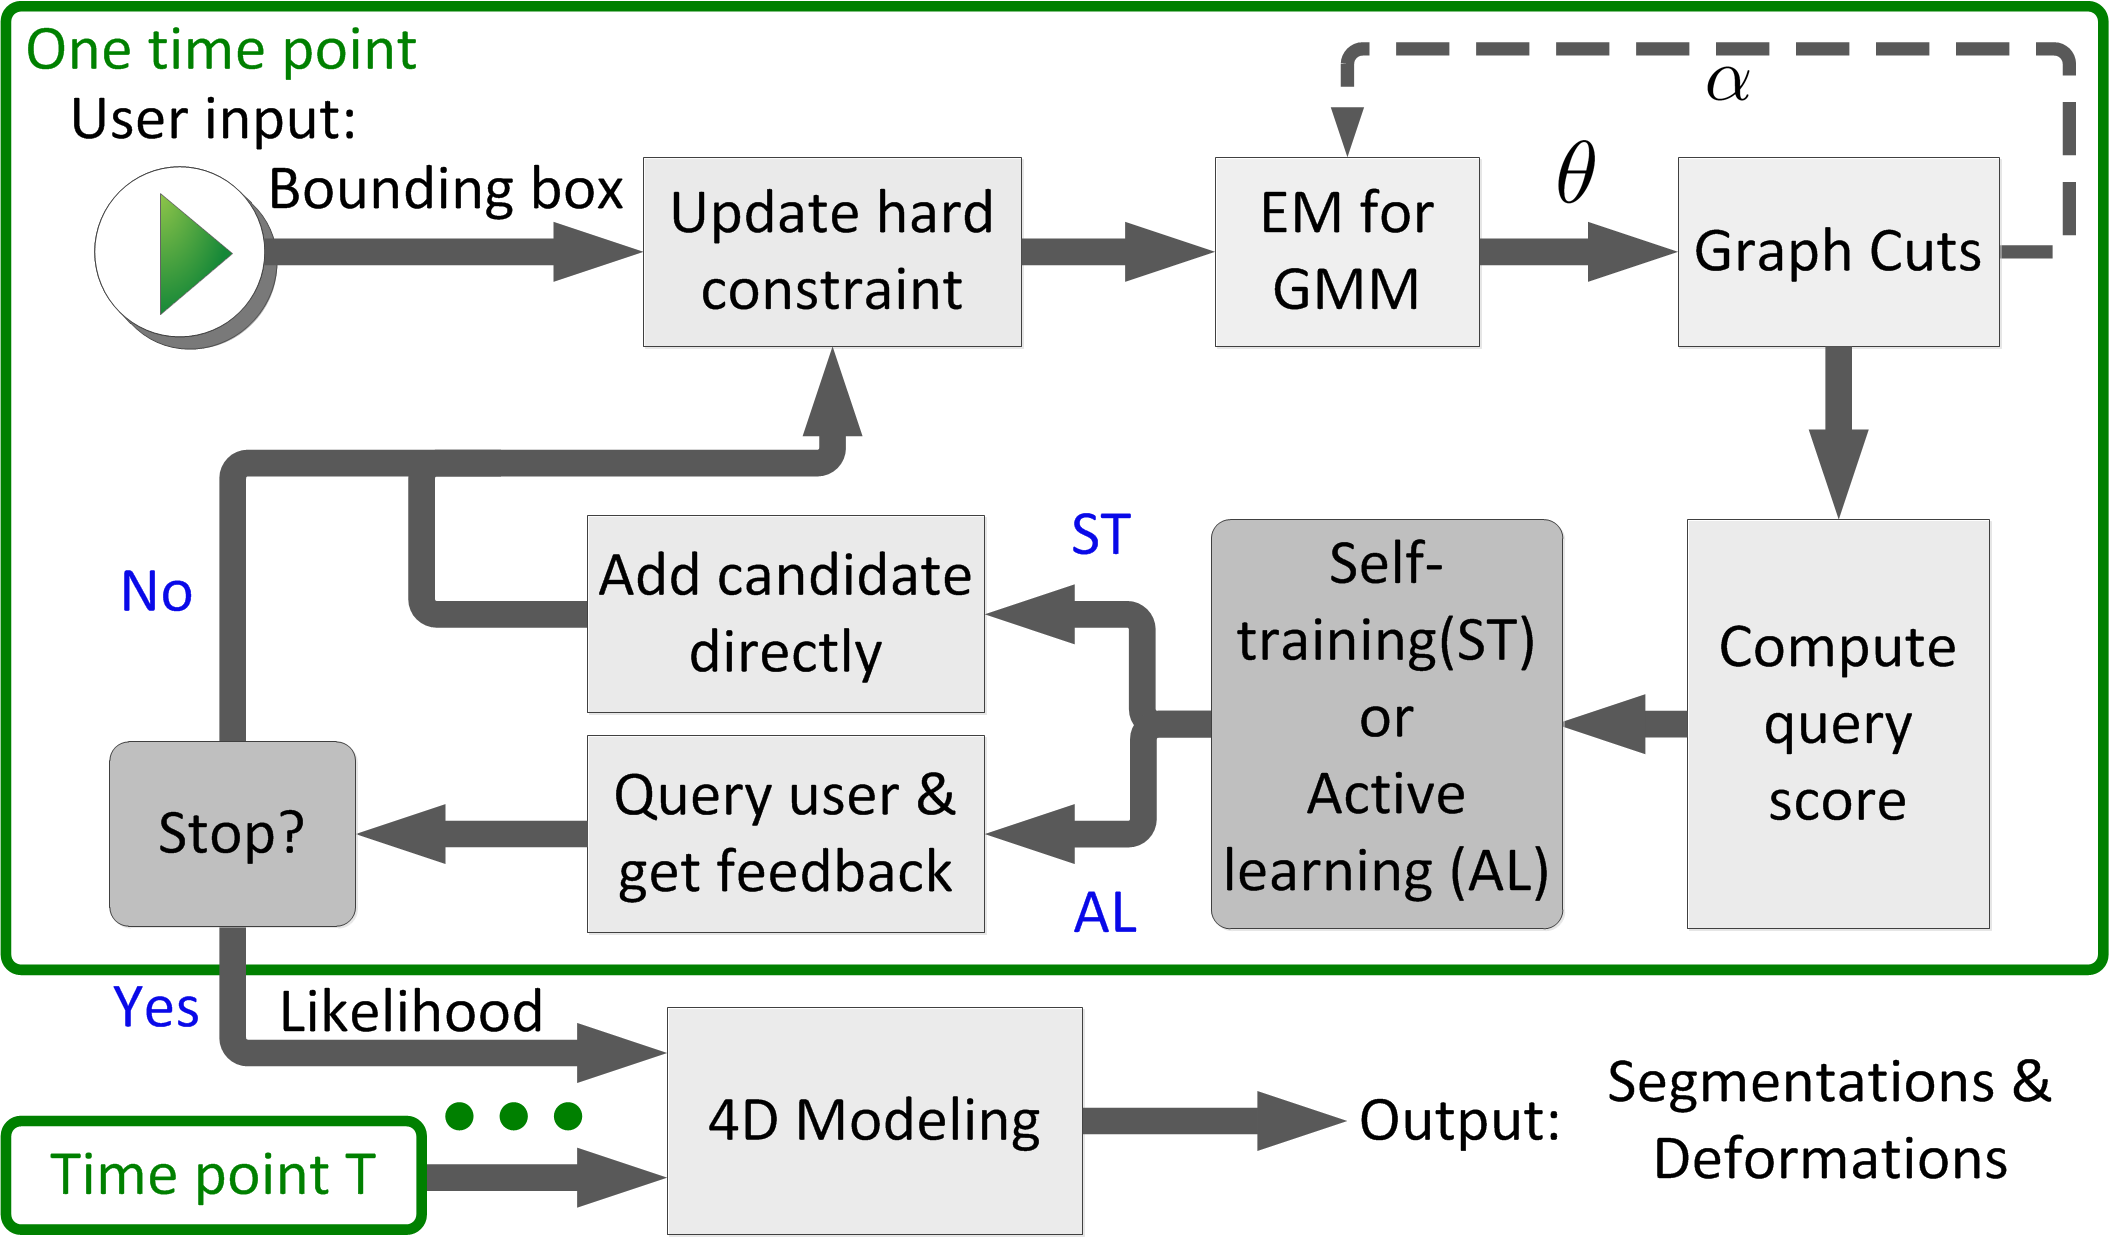
\includegraphics[width = 1\textwidth]{actlearn_fig/flowchart}
\end{frame}

\subsection{The Model}
\begin{frame}
\frametitle{A MRF Prior}
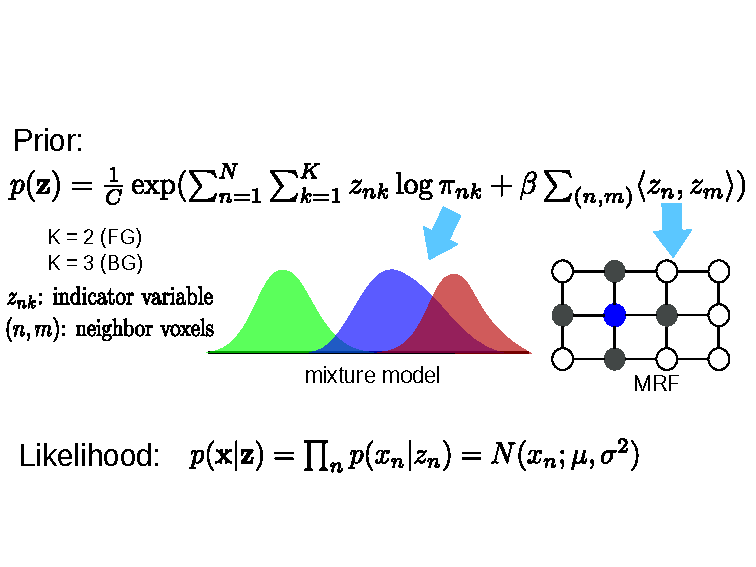
\includegraphics[width = 1\textwidth]{actlearn_fig/prior}
\end{frame}

\frame{\frametitle{Query Score}
 \begin{itemize}
 \item Voxel posterior $\rightarrow$ object query score.
  \item Prefer large objects, blob-like objects.
\end{itemize}

\begin{figure}
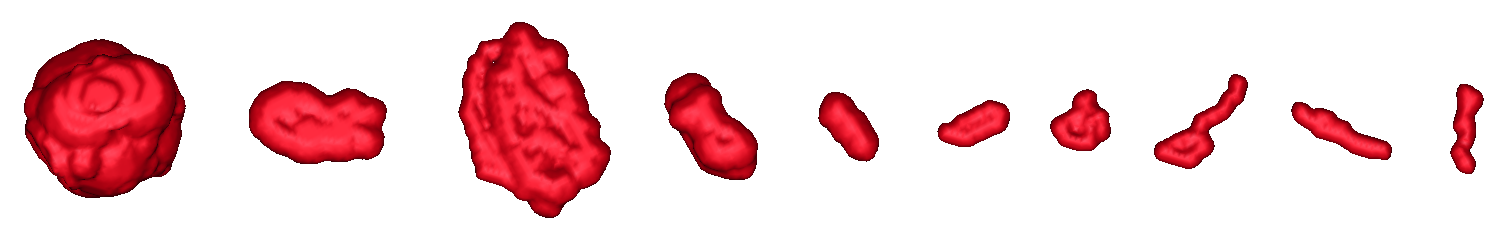
\includegraphics[width=1\textwidth]{actlearn_fig/All_candidate_patches_sorted}
\end{figure}

\begin{align*}
q(R_i) = \left (\sum_{n\in R_i} p(\alpha = 1| \vec x_n)  \right ) \Big /  \vert\{n: n\in \mathcal{B}(R_i) \}\vert.
\end{align*}
}

\subsection{Experiments}
\frame{\frametitle{Active Learning Iteration}
\begin{figure}
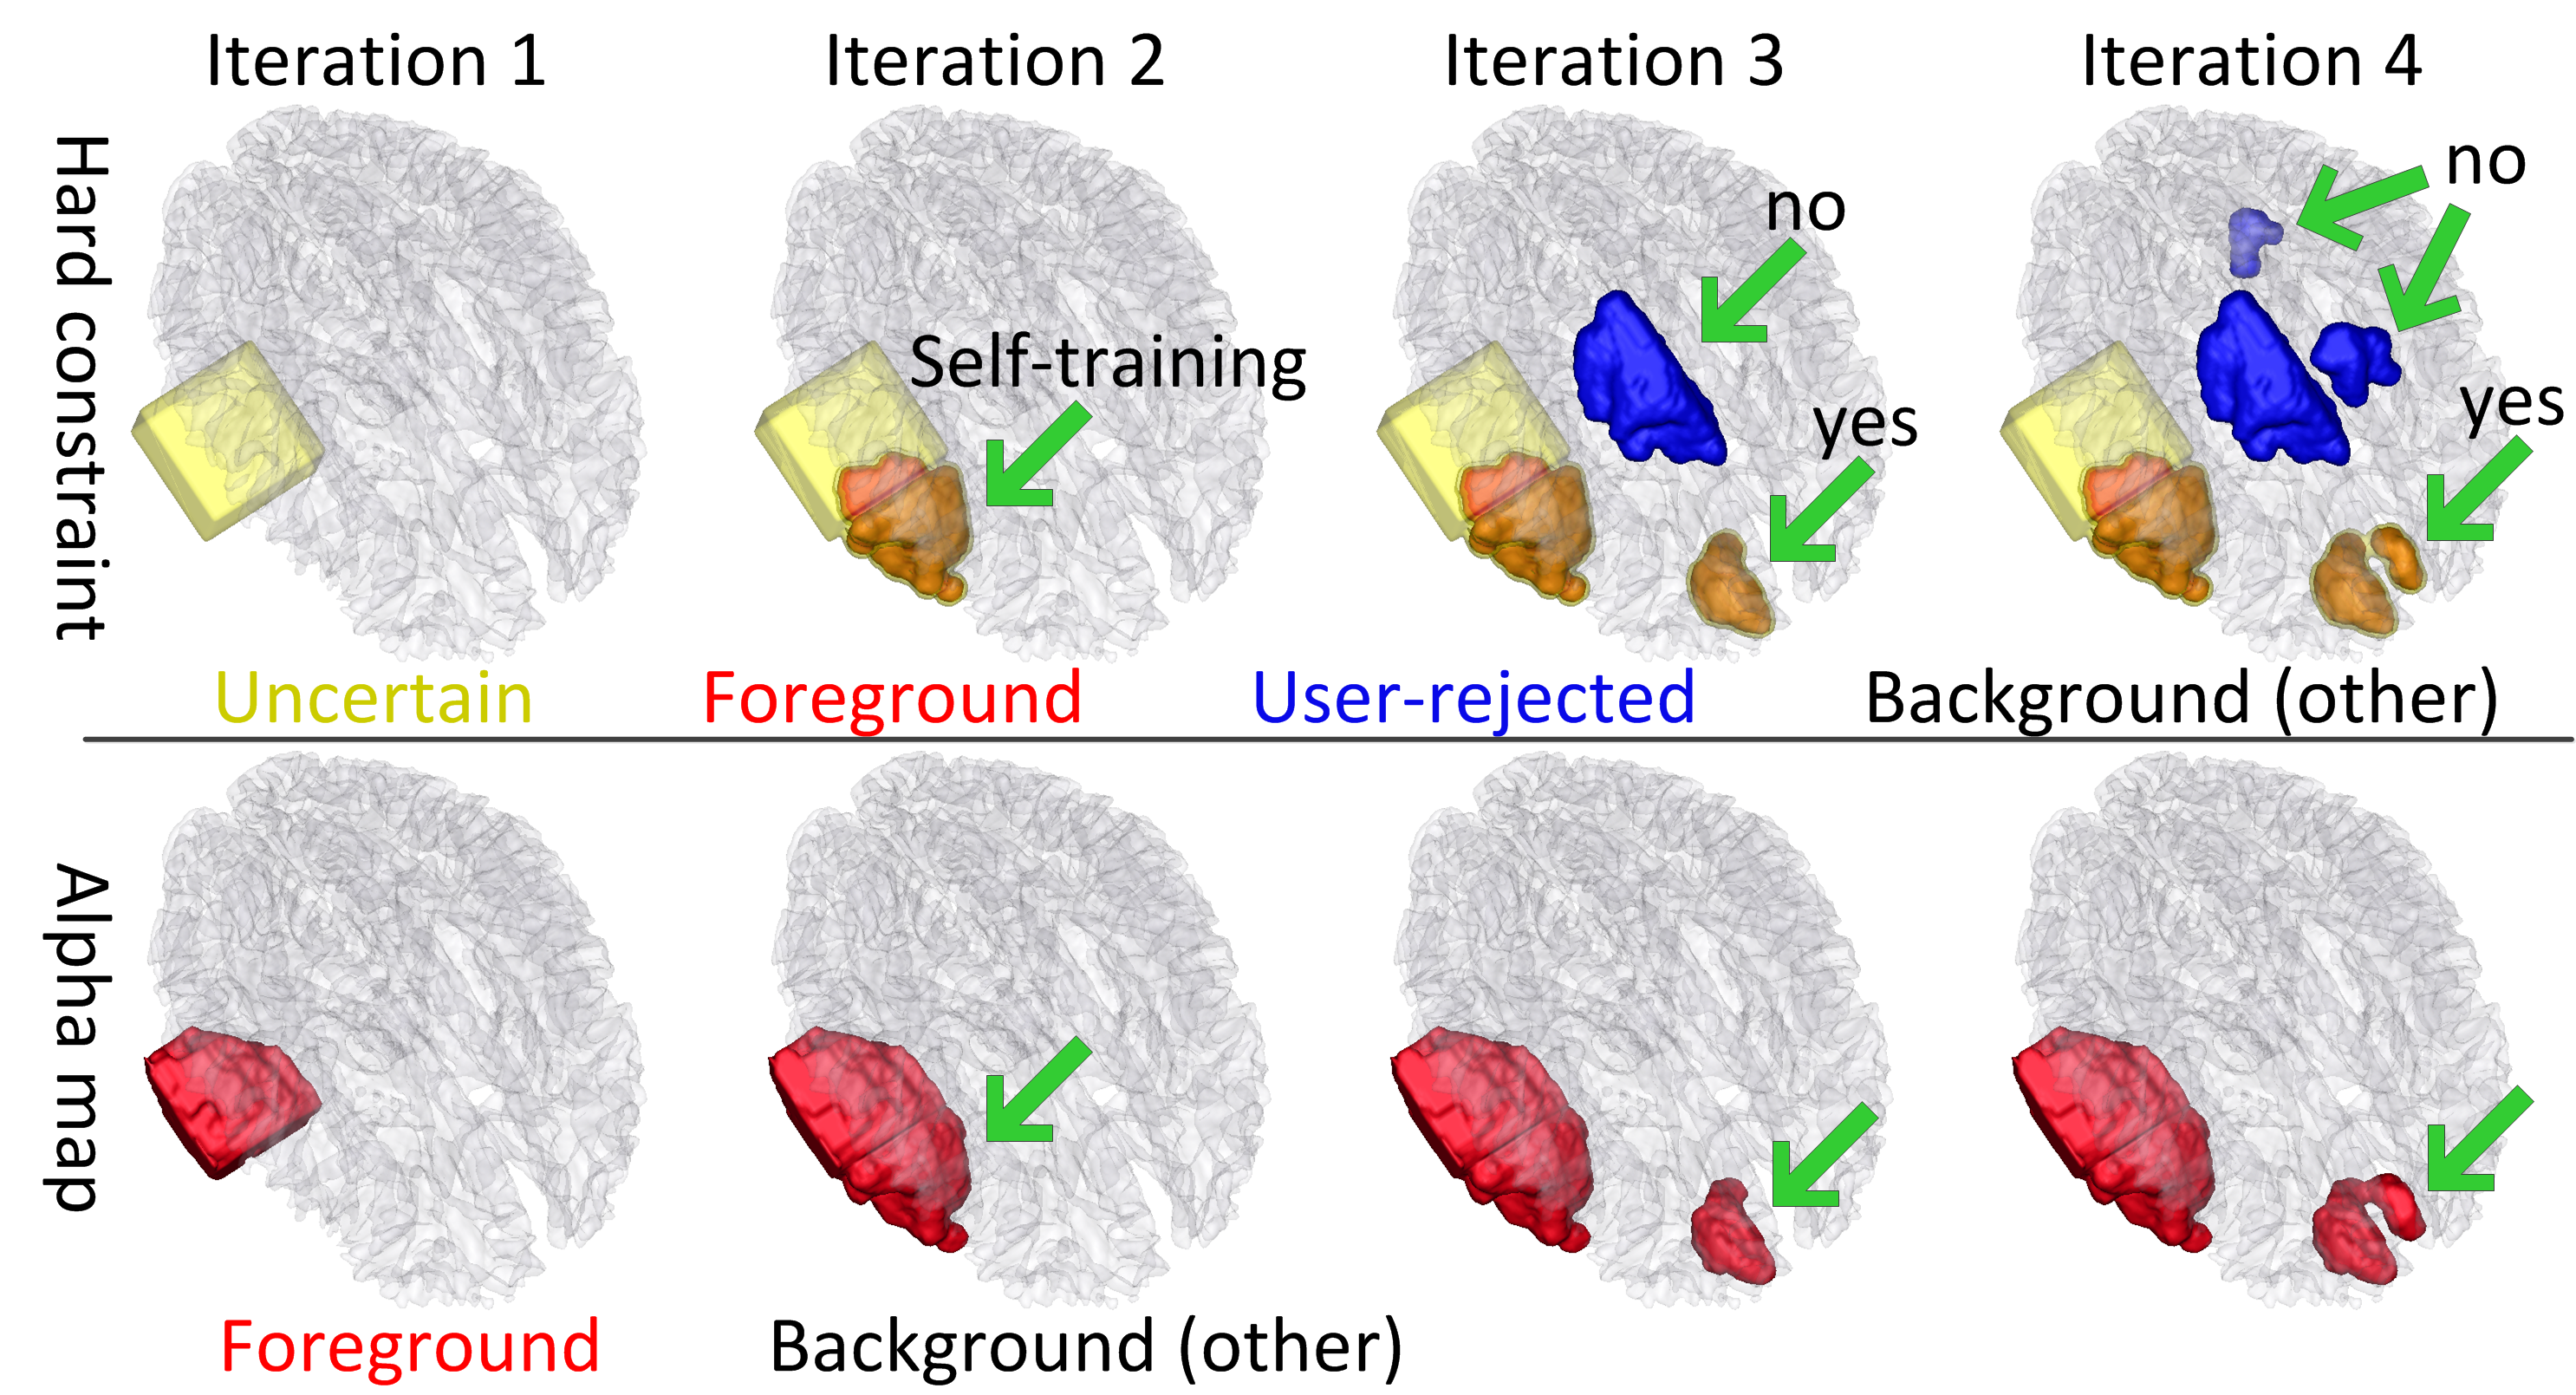
\includegraphics[width=1\textwidth]{actlearn_fig/iterative_process_new.png}
\end{figure}
}

\begin{frame}
\frametitle{Qualitative comparison}
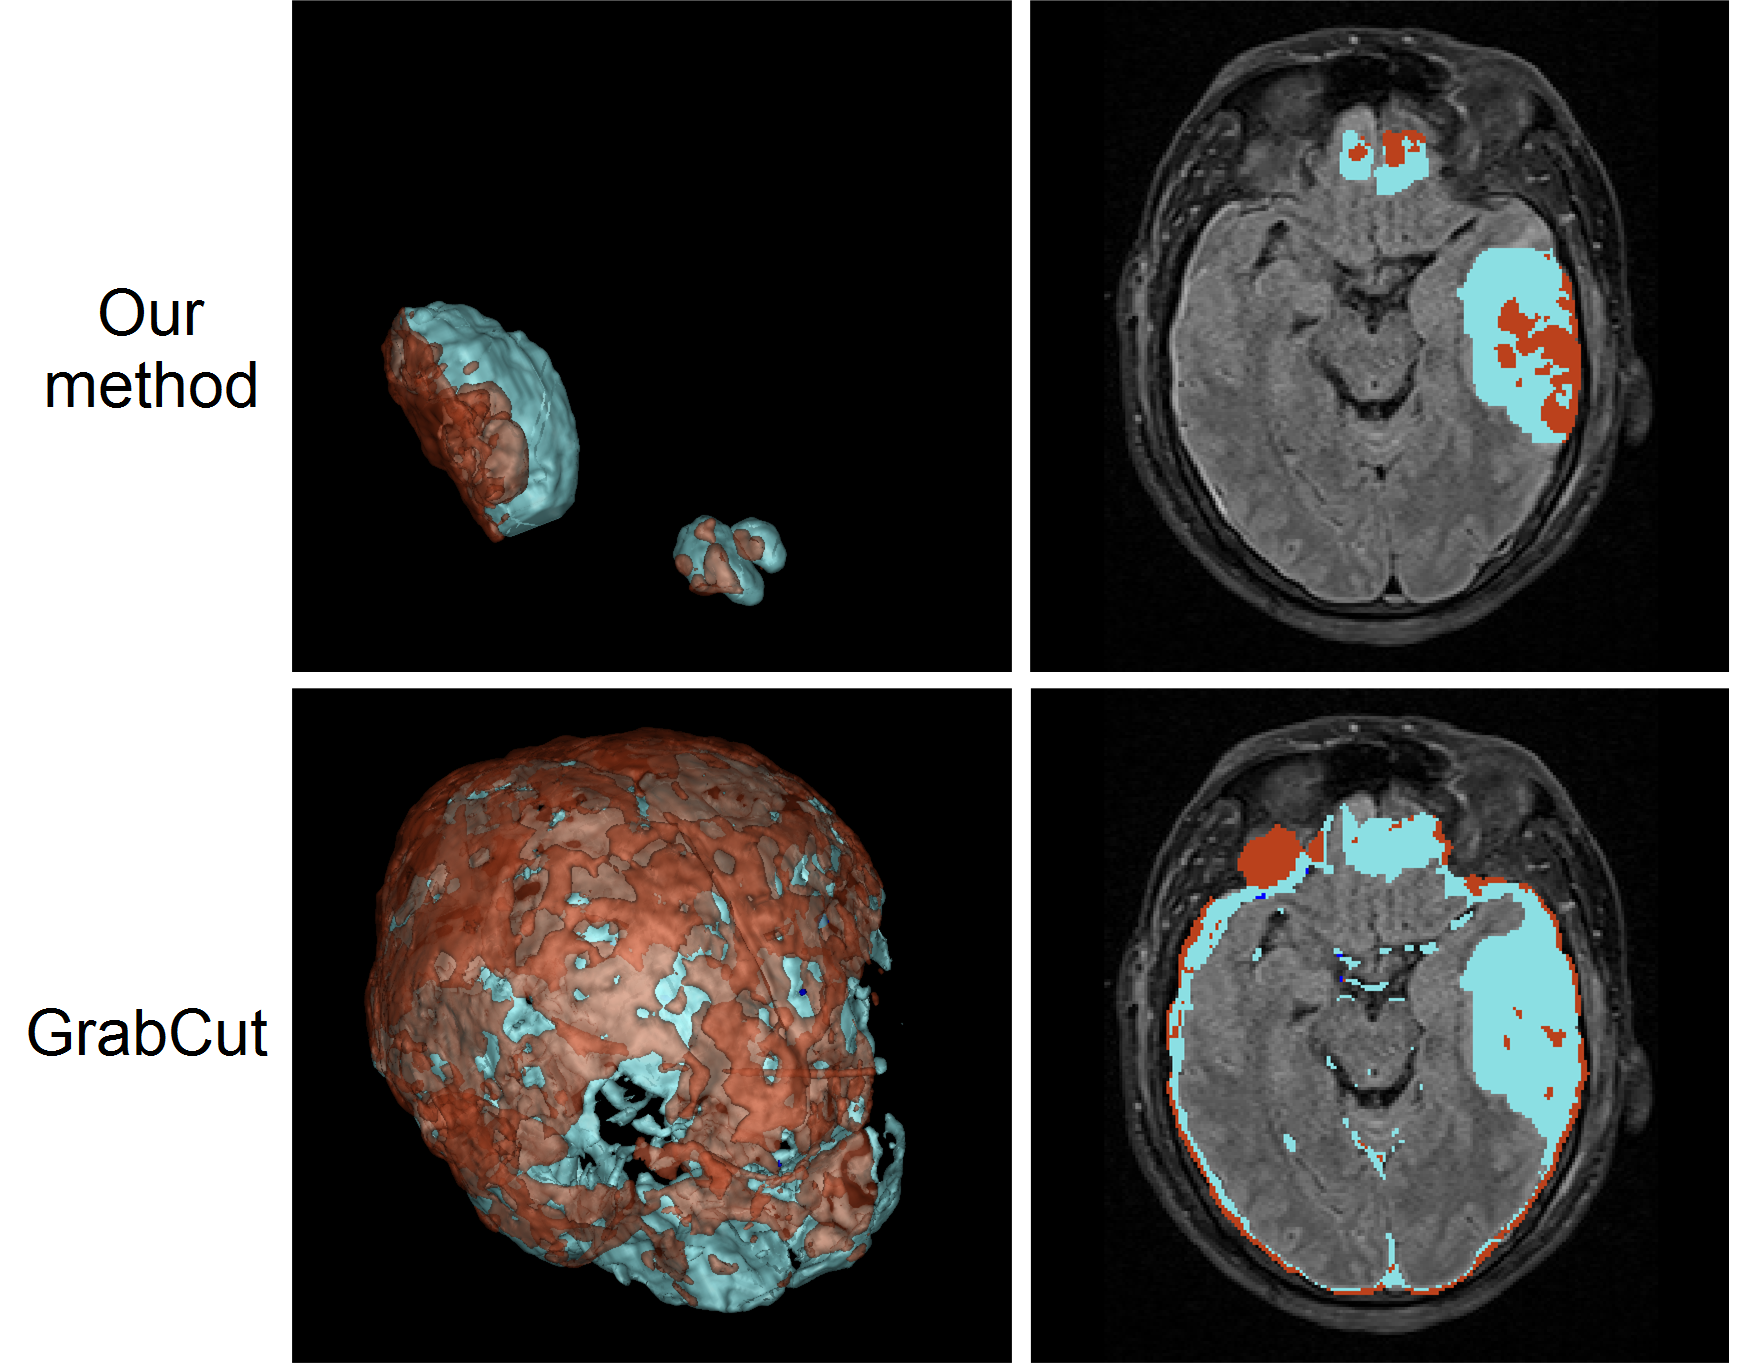
\includegraphics[width=0.99\textwidth]{actlearn_fig/qualitative_comp}
\end{frame}

\section{Conclusions}
\begin{frame}
  \frametitle{Conclusions}
  \begin{block}{}
    \begin{itemize}
    \item Graphical models (directed, undirected) are good for learning and
      inference of multivariate distribution.
    \item Model the within- and between-subject soft constraints for rs-fMRI.
    \item within- and between-class regularization for TBI segmentation.
    \item Other vision problem: Stereo matching, etc.
    \item Exact inference difficult. Approximate solution sufficiently good. 
    \end{itemize}
  \end{block}
\end{frame}

\begin{frame}
  \centering
  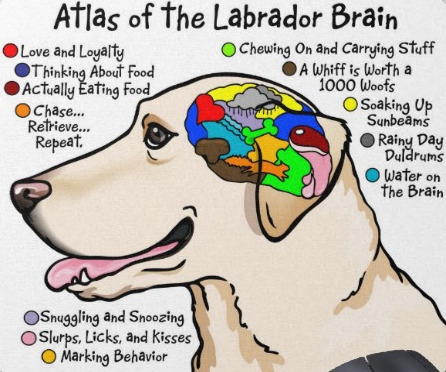
\includegraphics[width=0.5\textwidth]{sfig/dog_brain}\\
  \vspace{10pt}  
  Thank you.\\
  This is the end of the talk.
\end{frame}


%%%%%%%%%%%%%%%%%%%%%%%%%%%%%%%%%%%%%%%%%%%%%%%%%%%%%%%%%%%%%
%%%%%%%%%%%%%%%%%%%%%%%%%%%%%%%%%%%%%%%%%%%%%%%%%%%%%%%%%%%%%

\begin{frame}
\frametitle{Inter-Subject Consistency}
\begin{figure}
    \centering
      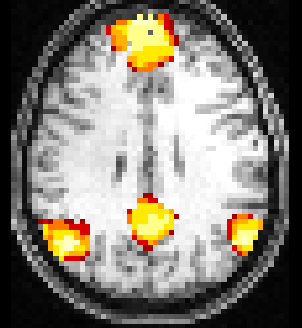
\includegraphics[height=0.14\textwidth]{figures_m2/mcem/dmn_a} 
      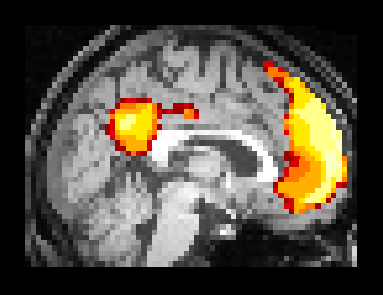
\includegraphics[height=0.14\textwidth]{figures_m2/mcem/dmn_s} 
      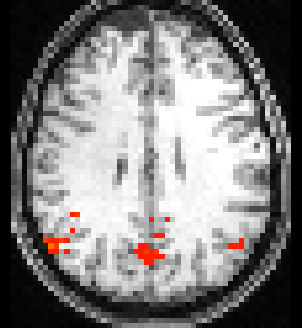
\includegraphics[height=0.14\textwidth]{figures_m2/ica_separate/DMN_a} 
      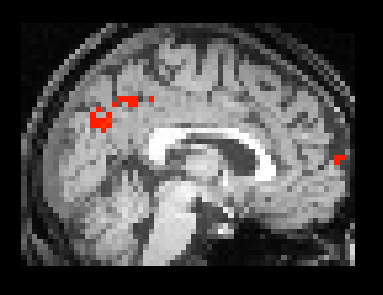
\includegraphics[height=0.14\textwidth]{figures_m2/ica_separate/DMN_s}
      \includegraphics[height=0.14\textwidth]{figures_m2/ica_single/dmn_a} 
      \includegraphics[height=0.14\textwidth]{figures_m2/ica_single/dmn_s} 
      


    \includegraphics[height=0.14\textwidth]{figures_m2/mcem/motor_a} 
    \includegraphics[height=0.14\textwidth]{figures_m2/mcem/motor_s} 
    \includegraphics[height=0.14\textwidth]{figures_m2/ica_separate/motor_a} 
    \includegraphics[height=0.14\textwidth]{figures_m2/ica_separate/motor_s}
    \includegraphics[height=0.14\textwidth]{figures_m2/ica_single/motor_a} 
    \includegraphics[height=0.14\textwidth]{figures_m2/ica_single/motor_s} 


    \includegraphics[height=0.14\textwidth]{figures_m2/mcem/visual_a} 
    \includegraphics[height=0.14\textwidth]{figures_m2/mcem/visual_s} 
    \includegraphics[height=0.14\textwidth]{figures_m2/ica_separate/visual_a} 
    \includegraphics[height=0.14\textwidth]{figures_m2/ica_separate/visual_s}
    \includegraphics[height=0.14\textwidth]{figures_m2/ica_single/visual_a} 
    \includegraphics[height=0.14\textwidth]{figures_m2/ica_single/visual_s} 


    \includegraphics[height=0.14\textwidth]{figures_m2/mcem/atten_a} 
    \includegraphics[height=0.14\textwidth]{figures_m2/mcem/atten_s} 
    \includegraphics[height=0.14\textwidth]{figures_m2/ica_separate/atten_a} 
    \includegraphics[height=0.14\textwidth]{figures_m2/ica_separate/atten_s}
    \includegraphics[height=0.14\textwidth]{figures_m2/ica_single/atten_a} 
    \includegraphics[height=0.14\textwidth]{figures_m2/ica_single/atten_s} 

  \caption{Comparison of the overlap of the label maps estimated by our MCEM
    approach, group ICA and single subject ICA on 16 subjects. Left: MCEM
    methods. Middle: single subject ICA. Right: group ICA. Color map ranges from
    8 (red) 16 (yellow). }
\end{figure}
\end{frame}


\begin{frame}
\frametitle{The Algorithm: MCEM Sampling on HMRF Model}
\begin{algorithm}[H]
  %% \SetAlgoLined
  \KwData{Normalized rs-fMRI, initial group label map}
  \KwResult{MC samples of label maps $\{X^m, m = 1, \dots, M\}$, parameters $\{\beta, \mu, \sigma\}$}
  \While{$\mathbb{E}_{P(Y|X)}[\log P(Y, X;\theta)]$ not converged}{
    %% E step\;
    \Repeat{$B+M$ times}{
      \lForEach(){$s \in \cV_G$}{
        Draw sample of $x_s$ from $P(x_s | x_{-s}, y_s;\theta)$
      }
      \ForEach(){$j  = 1\dots J$}{
        \lForEach(){$s \in \cV_j$}{
        Draw sample of $x_s$ from $P(x_s | x_{-s}, y_s; \theta)$
        }
      }
      Save sample $X^m $ after $B$ burn-ins\;
    }
    %% M step\;
    \ForEach{$l = 1\cdots L$} {
      Estimate $\{\mu_l, \kappa_l\}$ by maximizing $(1/M)\sum_{m=1}^M\log P (Y|X^m;\theta)$\;
    }
    Estimate $\beta$ by maximizing $(1/M)\sum_{m=1}^M\log P (X^m;\theta)$\;
  }
\end{algorithm}
\end{frame}

\begin{frame}
  \frametitle{Inter-level Links Estimation}
  \begin{columns}
    \begin{column}{0.55\textwidth}
      \begin{block}{Bayesian  Cross-Validation}
          $\alpha = \argmax P(Y_t|Y;\alpha, \theta_t)$ \\
          \begin{align*}
            &P(Y_t | Y;\alpha, \theta_t)\\
            &= \int P(Y_t | X_t; \theta_t) P(X_t| Y;\alpha)\, \textrm{d} X_t \\
            &\approx (1/M)\sum_m P(Y_t|X_t^m; \alpha, \theta_t),\\
            &\quad X_t^m \sim P(X_t|Y; \alpha).
          \end{align*}
          $X_t$'s are generated within MCEM.
        \end{block}
      \end{column}

    \begin{column}{0.45\textwidth}
      \includegraphics[width = 0.8\textwidth]{sfig/predictLLvsAlpha}
      \end{column}
    \end{columns}
\end{frame}

\begin{frame}
\frametitle{Bootstrapping: Subject Variance Maps}
\centering
\includegraphics[width = 1\textwidth]{sfig/sub_var}
\end{frame}

\begin{frame}
  \frametitle{Synthetic Data: Monte Carlo Test}
  \includegraphics[width = 1\textwidth]{sfig/2level_3smoothing}
\end{frame}

\end{document}
